\documentclass[a4paper,12pt,onepage,titlepage]{article}
\usepackage{report}
\usepackage{enumitem}
\usepackage{listings}

\graphicspath{ {images/} }
\begin{document}
\setcounter{secnumdepth}{4}

% Title page (Design in your own way)

\pagenumbering{gobble}

\begin{titlepage}
  \centering
  \large

  
\includegraphics[height=1.5in]{images/tu}\\
  {\Large\sc Tribhuvan University}\\
  {\Large\sc Institute of Engineering}\\
  {\Large\sc Pulchowk Campus}\\

  ~

  
  {\Huge\sc INTERACTIVE VOICE RESPONSE SYSTEM WITH SPEECH RECOGNITION}\\

  ~


  By:\\
  {\bf Prabin Bhandari} (070/BCT/525)\\
  {\bf Pujan Maharjan} (070/BCT/526)\\
  {\bf Raj Dangol} (070/BCT/529)\\
  {\bf Sagar Aryal} (070/BCT/534)\\

  ~

  \normalsize
  A PROJECT WAS SUBMITTED TO THE DEPARTMENT OF ELECTRONICS AND COMPUTER
  ENGINEERING IN PARTIAL FULLFILLMENT OF THE REQUIREMENT FOR THE BACHELOR'S
  DEGREE IN COMPUTER ENGINEERING
  ~

  ~
  
  DEPARTMENT OF ELECTRONICS AND COMPUTER ENGINEERING\\
  LALITPUR, NEPAL

  \vfill
  August, 2017

\end{titlepage}

\newpage
\phantomsection \addcontentsline{toc}{section}{LETTER OF APPROVAL}
\pagenumbering{roman}
\setcounter{page}{2}
{
  \centering

  TRIBHUVAN UNIVERSITY\\
  INSTITUTE OF ENGINEERING\\
  PULCHOWK CAMPUS\\
  DEPARTMENT OF ELECTRONICS AND COMPUTER ENGINEERING\\
}

~

The undersigned certify that they have read, and recommended to the Institute of
Engineering for acceptance, a project report entitled "Interactive Voice Response System With Speech Recognition" 
submitted by Prabin Bhandari, Pujan Maharjan, Raj Dangol, and Sagar Aryal
in partial fulfilment of the requirements for the Bachelor's degree in Computer Engineering.  

~

~

~

\begin{minipage}[t]{0.55\textwidth}
  \rule{2in}{1pt}\\
  Supervisor,\\
  Dr. Basanta Joshi,\\
  \small
  Department of Electronics \& Computer Engineering,\\
  Institute of Engineering, Pulchowk Campus,\\
  Tribhuvan University, Nepal
\end{minipage}
\hspace{0.5cm}
\begin{minipage}[t]{0.40\textwidth}
  \rule{2in}{1pt}\\
  Internal Examiner,\\
  Babu Ram Dawadi,\\
  Professor(Assistant),\\
 DOECE Pulcowk Campus, IOE, TU\\
\end{minipage}

~

~

~

\begin{minipage}[t]{0.55\textwidth}
  \rule{2in}{1pt}\\
  Dr. Diwakar Raj Pant,\\
  Head of Department,\\
  \small
  Department of Electronics \& Computer Engineering,\\
  Institute of Engineering, Pulchowk Campus,\\
  Tribhuvan University, Nepal
\end{minipage}
\hspace{0.5cm}
\begin{minipage}[t]{0.40\textwidth}
  \rule{2in}{1pt}\\
  External Examiner,\\
  Krishna Prasad Bhandari,\\
  Deputy Manager, Nepal Telecom,\\
  Bhadrakali Plaza, Kathmandu\\
\end{minipage}
~

~

~
~

~
{\bf Date of Approval} ...............\\
\end{document}

\newpage
\phantomsection \addcontentsline{toc}{section}{COPYRIGHT}

\section*{COPYRIGHT}

The author has agreed that the Library, Department of Electronics and Computer Engineering, Pulchowk Campus, Institute of Engineering may make
this report freely available for inspection. Moreover, the author has agreed that permission for extensive copying of this project report for 
scholarly purpose may be granted by the supervisors who supervised the project work recorded herein or, in their absence, by the Head of the 
Department wherein the project report was done. It is understood that the recognition will be given to the author of this report and to the 
Department of Electronics and Computer Engineering, Pulchowk Campus, Institute of Engineering in any use of the material of this project report. 
Copying or publication or the other use of this report for financial gain without approval of to the Department of Electronics and 
Computer Engineering, Pulchowk Campus, Institute of Engineering and author\textquotesingle s written permission is prohibited.

Request for permission to copy or to make any other use of the material in this report in whole or in part should be addressed to:\\

Head\\
Department of Electronics and Computer Engineering\\
Pulchowk Campus, Institute of Engineering\\
Lalitpur, Kathmandu\\
Nepal\\


\newpage
\phantomsection \addcontentsline{toc}{section}{ACKNOWLEDGEMENTS}

\section*{ACKNOWLEDGEMENTS}

First of all, we would like to take this opportunity to express our sincere gratitude to the Department of Electronics and Computer Engineering, Pulchowk Campus for providing us the opportunity to undertake this project by including it as a part of curruculum in B.E. Computer Engineering. We are extremely thankful to Dr. Basanta Joshi, our Project Supervisor for providing us with his invaluable guidance and support throughout every phase of the project development. His useful suggestions and continuous motivation are sincerely acknowledged. We would also like to express our gratitude to our teachers and colleagues whose support and suggestions have been an invaluable contribution.Their continuous encouragement and valuable comments are truly appreciable.

Lastly, a very special thanks to all the people who are involved directly and indirectly in the contribution of the project in many ways and helped for the completion of the project in time.

Prabin Bhandari (070/BCT/525)\\
Pujan Maharjan (070/BCT/526)\\
Raj Dangol (070/BCT/529) \\
Sagar Aryal (070/BCT/534) \\




\newpage
\phantomsection \addcontentsline{toc}{section}{ABSTRACT}

\section*{ABSTRACT}


This report represents the report on a project entitled "Interactive Voice Response System with Speech Recognition" as a part of the curriculum for the final year project of B.E. in Computer Engineering. The report discusses various methods and implementation techniques to build the system of IVR system with speech recognition and presents the results of the system being implemented. \\
The project entitled "Interactive Voice Response System with Speech Recognition" is an Interactive Voice Response (IVR) system with the capability of Speech Recognition. The project focuses on a system where the user interacts with the system with his/her voice and on the basis of the user's voice input the system performs various actions as a response to the voice command.It is an approach to make use of the voice of the user to recognize the given command.The project is helpful for various large organizations where there are many call queries or for telecommunications companies or other business ventures where user queries through their voice online or via cellular connections.  The prime focus of the project is to develop an application environment whereby users speech request are being processed for further task accomplishment as per the request.The final system being developed is a system being capable to take a real time voice input from a user under certain domain range and in response the system performs a task related to input.




{\setlength{\parskip}{0pt}
  % Table of contents
  \newpage
  \phantomsection\addcontentsline{toc}{section}{TABLE OF CONTENTS}
  \renewcommand{\contentsname}{TABLE OF CONTENTS}
  \tableofcontents

  % List of figures
  \newpage
  \phantomsection\addcontentsline{toc}{section}{LIST OF FIGURES}
  \renewcommand{\listfigurename}{LIST OF FIGURES}
  \listoffigures


  % List of SYMBOLS AND ABBREVIATIONS 
  \newpage
  \renewcommand{\listtablename}{LIST OF SYMBOLS AND ABBREVIATIONS}
  \phantomsection\addcontentsline{toc}{section}{LIST OF ABBREVIATIONS}
\section*{LIST OF ABBREVIATIONS}

{
  \renewcommand{\arraystretch}{1.1}

  \begin{tabular}{ll}
    \textbf{AI} & Artificial Intelligence \\
    \textbf{ANN} & Artificial Neural Network \\
	\textbf{ASR} & Automatic Speech Recognition \\
	\textbf{AVR} & Automatic Voice Recognition \\
	\textbf{DFT} & Discrete Fourier Transform \\
	\textbf{FFT} & Fast Fourier Transform \\
	\textbf{GPU} & Graphical Processing Units \\ 
	\textbf{GRU} & Gated Recurrent Unit \\
	\textbf{HMM} & Hidden Markov Model \\   
	\textbf{IFFT} & Inverse Fourier Transform \\
	\textbf{IVR} & Interactive Voice Response \\
	\textbf{LPC} & Linear predictive coding \\
	\textbf{LSTM} & Long Short Term Memory \\
	\textbf{MFCC} & Mel-Frequency Cepstral Coefficients \\	
    \textbf{RNN} & Recurrent Neural Network \\
      
  \end{tabular}
}


}

\newpage\pagenumbering{arabic} % Start arabic page numbers from here


\section{INTRODUCTION}


\subsection{Background}

Speech probably is the most efficient and natural way to communicate with each other. Thus, being the best way of communication, it could also be a useful interface to communicate with machines and systems like IVR system. The Interactive Voice Response (IVR) system along with the speech recognition technology can play efficient role in providing easy and efficient customer/user service. If properly implemented it can increase the user satisfaction and offer new services. Speech Recognition has now begun to dominate the market technology and is pushing away the traditional way of using hectic interfaces such as keyboards and mouse as input source to computer system. Voice command based applications will make life easier due to the fact that people will get easy and fast access to information. Therefore the popularity of automatic speech recognition system has been greatly increased. The work of speech recognition further helps in establishing  an easy way communication between interactive response system and users/ customers i.e. as a part of post processing of the speech recognizing process we can accomplish some computational task with such a system making voice input as a trigger to do some task within the system.


\setlength{\parindent}{1cm}The IVR with AVR (Automatic Voice Recognition) allows callers to obtain information and perform transactions simply by speaking naturally. Recognition of free-form conversation is not yet a reality, and speech recognition has sometimes been over-hyped in the past. However, speech recognition technology is now proving itself commercially viable in a number of customer service applications.Early speaker-dependent dictation systems had to be trained to understand the speech of one specific user. Now, speaker-independent recognition technologies allow IVR systems to interpret the speech of many users. Today's speech-enabled IVR applications serve large numbers of unknown callers without prior training of the system. Many factors are driving the emergence of speech as the IVR user interface of choice for today and tomorrow. The first is reducing labor costs. The cost of employing live customer service agents is rising at the same time that organizations are facing increased pressure to reduce the cost of serving customers. When an automated call-processing solution must be employed, a speech-enabled IVR application increases caller acceptance because it provides the friendliest and fastest self-service alternative to speaking with a customer service agent. 

In this project our focus is to build such an application where users can simply command the IVR system with their voice and in response the system accomplishes its task as per the user request. The system could have wide range of application in various fields such as interactive response customer support center, automatic number dialer, banking assistant etc.


\subsection{Problem Statement}

Most of the works done till today on the field of IVR system has been primarily focused on the input mechanisms based on the keyboard or touch pad. In such cases it is tedious to provide the input command every time through typing of texts. This way of providing input to the computer system may be enhanced if we could provide direct speech input instead of typing. This enables in fast interaction between the system and user and therefore increases overall satisfaction of the customers. This also increases the speed of access of the information from the system.
Furthermore, English language has been widely implemented in IVR systems. This has created difficulty for people while interacting with the system. Thus by implementing the Nepali voice commands it is easier to interact and provide the input to the system.


The major focus of the project being developed is the use of direct Nepali voice command for the interactive voice response system without need of typing which then further can be applicable to real world applications like call centers, customer support systems and other several organization inquiry systems.

\subsection{Objectives}
\subsubsection{Project objectives}

The prime objective of the project being proposed is to design and build a system that a basic user can interact so that she/he can make use of voice commands to deal with system i.e. making a system that has capability of recognizing the isolated speaker words and process the request to forward the given task.

The typical objectives are listed below:
\begin{itemize}
	\item To make use of domain specific models and algorithms in field of speech recognition.
	\item To develop an interactive voice response system along with speech recognition attribute.
	\item To understand the basics of speech processing.
	\item To get knowledge on various speech recognition approaches.
	\item To get insights on speech responsive application development.
\end{itemize}

\subsubsection{Academic objectives}
Academically, the project is primarily focused on fulfilling the discipline of an engineering student as a computer engineer working on a project and gain experience as a team throughout the different phases of a project. Some Typical academic objectives of the project are :
\begin{itemize}
	\item To fulfill the requirements of the major project of B.E. in computer engineering.
	\item To design and complete a functional project that integrates various course concepts.
	\item To develop various skills related to project management like team work, resource management, documentation and time management.
	\item To get hands-on experience of working in a project as a team work.
	\item To learn about and become familiar with the professional engineering practices.
\end{itemize}
\subsection{Scope}
Interactive Voice Response (IVR) system is being more popular day by day. Such systems make it more convenient in interaction with the user and computer system and hence help in easy accomplishment of several tasks. The IVR system serves as a bridge between people and computer system. The IVR system with Automatic Voice Recognition (AVR) can make it more convenient for the users if they can command the system through their voice and this makes such system applicable in vast areas.The current system is being built for the desktop computers and won't be implemented in actual phone devices due limitation of time and research. However in future the project work can be further enhanced and has huge scope and potential for future implementations in several areas. Some of the applicable areas are discussed as follows:
\begin{itemize}
	\item Organizational inquiry desk: The system can be used in several organization for easy information access regarding the organization using the voice command.
	\item Automatic speech to text conversion: The proposed system deals only with the isolated words detection but with further enhancement in algorithms it can be used in speech to text conversion application.
	\item Speech controlled applications: we can make use of speech recognition of Nepali words in performing the task of new developed applications and hence make more user friendly applications.
	\item Speech control in embedded systems: using speech recognition technology several tasks can be controlled using voice commands in embedded systems this further increases the automation of works and hence can be very beneficial in industrial process automation.
	\item Application for Disabled people: Disabled people are another part of the population that can use speech recognition programs. It is especially useful for people who can't use their hands, from the profoundly physically impaired to people with mild repetitive stress injuries i.e. persons who might require helpers to control their environments.
\end{itemize}


\newpage
\section{LITERATURE REVIEW}

\subsection{Historical Overview of Speech Recognition}
The concept of speech recognition started somewhere in 1940s, practically the first speech recognition program appeared in 1952 at the bell labs, that was about recognition of a digit in a noise free environment. 1940s and 1950s consider as the foundational period of the speech recognition technology, in this period work was done on the foundational paradigms of the speech recognition that is automation and information theoretic models. In the 1960s, it was able to recognize small vocabularies (order of 10-100words) of isolated words, based on simple acoustic-phonetic properties of speech sounds. The key technologies that were developed during this decade were, filter banks and time normalization methods. In 1970s the medium vocabularies (order of 100-1000 words) using simple template-based, pattern recognition methods were recognized. In 1980s large vocabularies (1000-unlimited) were used and speech recognition problems based on statistical, with a large range of networks for handling language structures were addressed. The key invention of this era were   model (HMM) and the stochastic language model, which together enabled powerful new methods for handling continuous speech recognition problem efficiently and with high performance. In 1990s the key technologies developed during this period were the methods for stochastic language understanding, statistical learning of acoustic and language models, and the methods for implementation of large vocabulary speech understanding systems. After the five decades of research, the speech recognition technology has finally entered marketplace, benefiting the users in variety of ways. The challenge of designing machine that truly functions like an intelligent human is still a major one going forward.

\subsection{Speech Recognition Overview}
Speech Recognition (SR) is the process of extracting the string of words automatically from the speech signal, by means of an algorithm. It is the ability of a machine or program to identify words and phrases in spoken language and convert them to a machine readable format. Speech recognition is a powerful tool of the information exchange using the acoustic signal. Therefore, not surprisingly, the speech signal is for several centuries the subject of research. Speech recognition is a technology that makes a computer able to capture the words spoken by a human with a help of microphone. These words are later on recognized by speech recognizer, and in the end, system outputs the recognized words which can also serve as input to the further systems to accomplish several task. Speech recognition is basically the science of talking with the computer, and having it correctly recognized. Speech recognition is getting the meaning of an utterance such that one can respond properly whether or not one has correctly recognized all of the words. ASR has always been considered as an important bridge in fostering better human to human and human to machine communication. In the past, however, speech never actually became an important modality in the human to machine communication. This is partly because the technology at that time was not good enough to pass the usable bar for most real world users under most real usage conditions, and partly because in many situations alternative communication modalities such as keyboard and mouse significantly outperform speech in the communication efficiency, restriction, and accuracy. In the recent years, speech technology started to change the way we live and work and became one of the primary means for humans to interact with some devices. This trend started due to the progress made in several key areas. First, Moor's law continues to function. The computational power available today, through multi-core processors, general purpose graphical processing units (GPUs), and CPU/GPU clusters, is several orders of magnitude more than that available just a decade ago. This makes training of more powerful yet complex models possible. These more computation demanding models significantly reduced the error rates of the ASR systems. Second, we can now access to much more data than before, thanks to the continued advance of the Internet and the cloud computing. By building models on big data collected from the real usage scenarios, we can eliminate many model assumptions made before and make systems more robust. Third, mobile devices, wearable devices, intelligent living room devices, and in vehicle infotainment systems became popular. On these devices and systems, alternative interaction modalities such as keyboard and mouse are less convenient than that in the personal computers. Speech, which is the natural way of human to human communication and a skill that majority of people already have, thus becomes a more favorable interaction modality on these devices and systems.



\subsection{Human Ear and Speech Recognition}
Humans are more effective than machines at recognizing speech. This advantage for
human listeners is particularly pronounced for speech that is heard against
background noise, contains unfamiliar words or is degraded in other ways. Yet,
automatic speech recognition (ASR) systems have made substantial advances over the
past few decades and are now in everyday use by millions of people around the world.
Until the performance of automatic speech recognition (ASR)  surpasses human
performance in accuracy and robustness, we stand to gain by understanding the basic 
principles behind human speech recognition (HSR).
In this section we provide a brief explanation of how human hearing works and 
how it is modeled. We will discuss in brief the functionality of several
components and try to understand the relation of it with the speech recognition systems.

\subsubsection{Human Hearing system}

The main function of hearing system is to get information about the outside, which is
carried by pressure variations in the air, that is, sound wave. Sound waves are
generated by the movement or vibration of an object, that is, sound source. As the
vibrating object moves out and in, the nearby air molecules create a slight increase
and decrease in pressure, called condensation and rarefaction, respectively. From the
pressure variations, we perceive what the sound source is and where it comes from.
We perceive a sound wave, which is a continual time series signal, by the ears.
We also perceive three-dimensional acoustic space by the ears, mainly because the
head-related transfer function (HRTF) between a point of a sound source and
the two ear entrances has directional characteristics from the shapes of the head and
the pinna. The pinna significantly modify the incoming sound, particularly at
high frequencies, and this is important in our ability for sound localization.After 
a sound wave arrives nearby, it passes through the peripheral auditory system, 
the outer ear, middle ear, and inner ear.
\begin{figure}[h]
	\begin{center}
		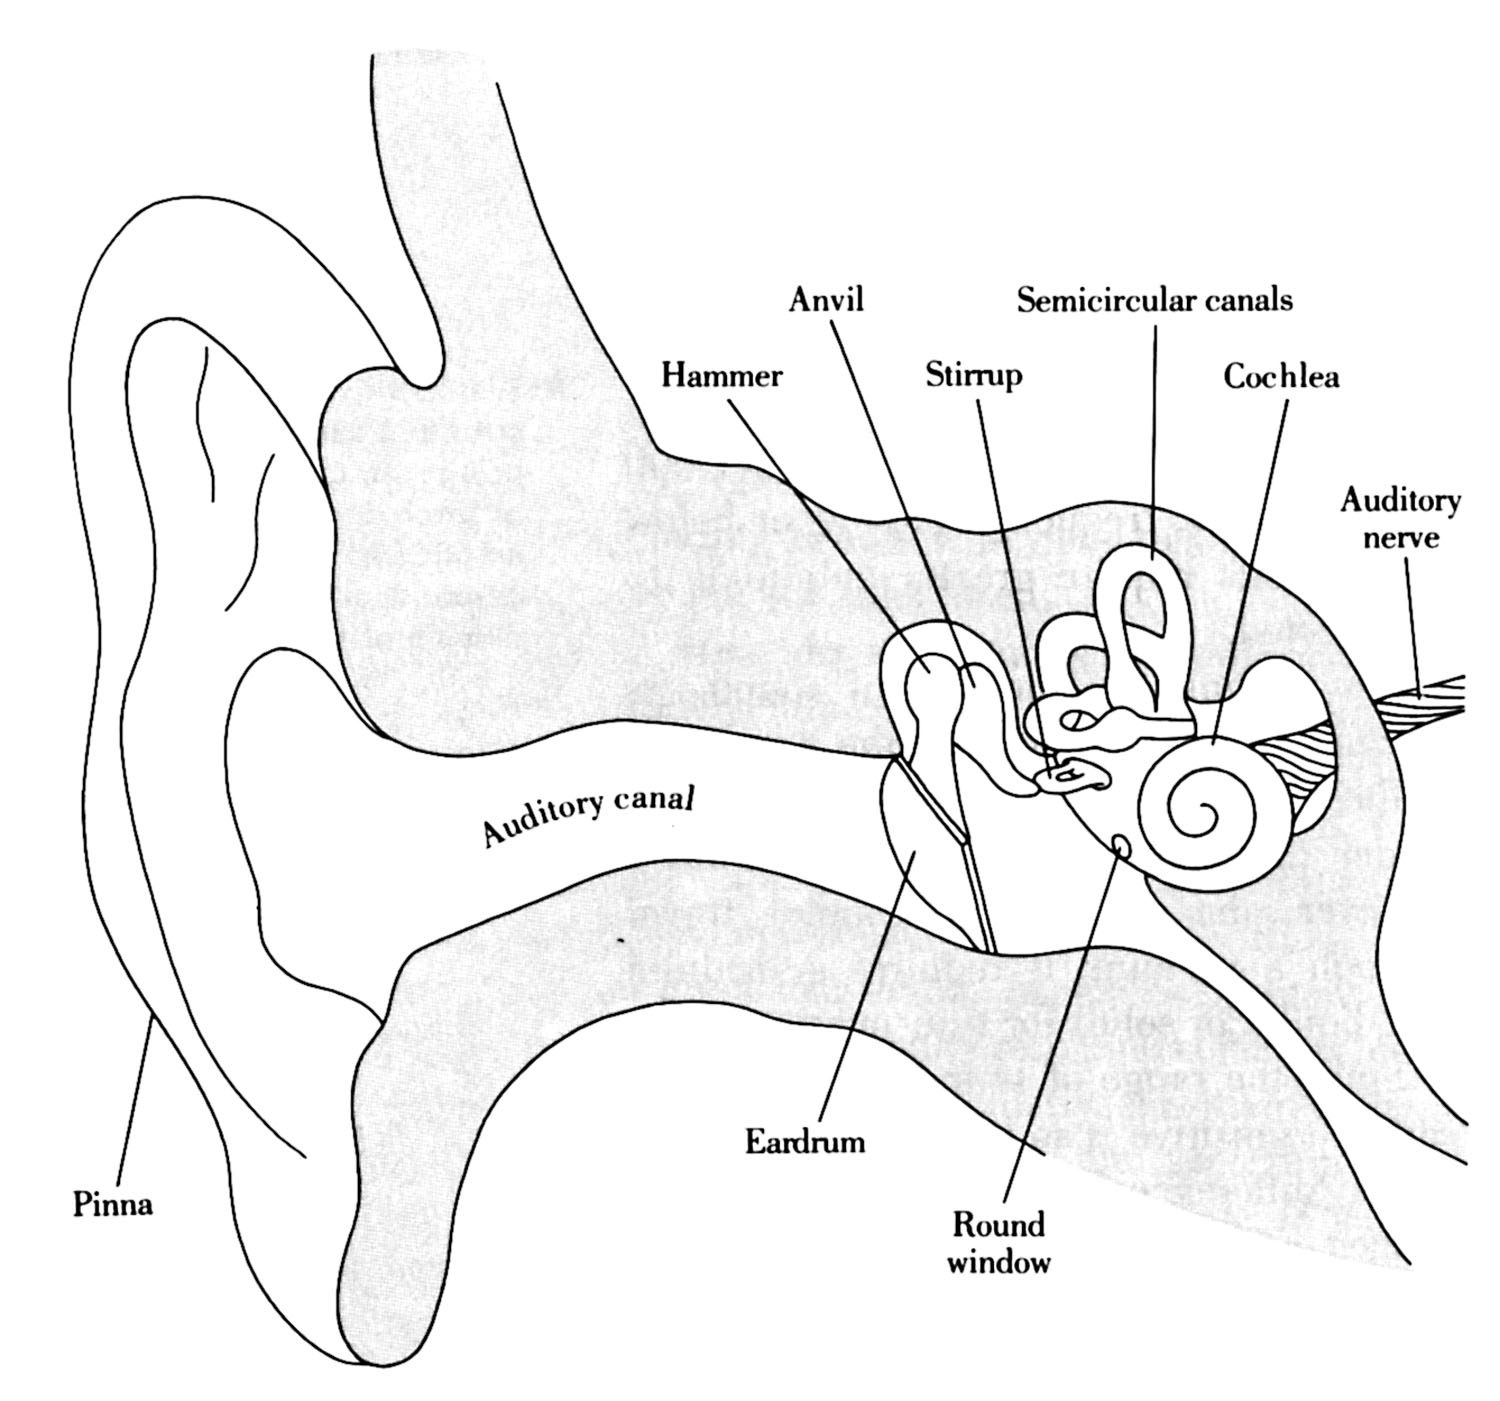
\includegraphics[scale=0.8]{images/ear_clear.jpg}
		\caption{Human Ear Hearing System}
	\end{center}
\end{figure} 

\vfill
\begin{enumerate}
	\item The Outer Ear
	
	The outer ear is the external part of the auditory system, including the pinna 
	and the ear canal. Sound travels down the ear canal and causes the eardrum, 
	or tympanic membrane, to vibrate. Because of the resonance of the outer ear, 
	we are more sensitive to sound frequencies between 1000 and 6000 Hz.
	The pinna is the only visible part of the ear (the auricle) with its special helical shape. It is the first part of the ear that reacts with sound. The function of the pinna is to act as a kind of funnel which assists in directing the sound further into the ear. Without this funnel the sound waves would take a more direct route into the auditory canal. This would be both difficult and wasteful as much of the sound would be lost making it harder to hear and understand the sounds. The pinna is essential due to the difference in pressure inside and outside the ear. The resistance of the air is higher inside the ear than outside because the air inside the ear is compressed and thus under greater pressure.
	In order for the sound waves to enter the ear in the best possible way the resistance must not be too high. This is where the pinna helps by overcoming the difference in pressure inside and outside the ear. The pinna functions as a kind of intermediate link which makes the transition smoother and less brutal allowing more sound to pass into the auditory canal (meatus).Once the sound waves have passed the pinna, they move two to three centimetres into the auditory canal before hitting the eardrum, also known as the tympanic membrane. The function of the ear canal is to transmit sound from the pinna to the eardrum. The eardrum (tympanic membrane), is a membrane at the end of the auditory canal and marks the beginning of the middle ear. The eardrum is extremely sensitive and pressure from sound waves makes the eardrum vibrate.  The auditory canal  functions as a natural hearing aid which automatically amplifies low and less penetrating sounds of the human voice. In this way the ear compensates for some of the weaknesses of the human voice, and makes it easier to hear and understand ordinary conversation.
	
	\item The Middle Ear
	
	The middle ear is the part of the ear between the eardrum and the oval window. The middle ear transmits sound from the outer ear to the inner ear. The middle ear consists of three bones: the hammer (malleus), the anvil (incus) and the stirrup (stapes), the oval window, the round window and the Eustrachian tube.The eardrum is very thin, measures approximately eight to ten millimeter in diameter and is stretched by means of small muscles. The pressure from sound waves makes the eardrum vibrate. The vibrations are transmitted further into the ear via three bones in the middle ear. These three bones form a kind of bridge, and the stirrup, which is the last bone that sounds reach, is connected to the oval window.
	The oval window is a membrane covering the entrance to the cochlea in the inner ear. When the eardrum vibrates, the sound waves travel via the hammer and anvil to the stirrup and then on to the oval window.
	When the sound waves are transmitted from the eardrum to the oval window, the middle ear is functioning as an acoustic transformer amplifying the sound waves before they move on into the inner ear. The pressure of the sound waves on the oval window is some 20 times higher than on the eardrum.
	
	
	\setlength{\parindent}{1cm}
	\setlength{\parskip}{1.1em}The pressure is increased due to the difference in size between the relatively large surface of the eardrum and the smaller surface of the oval window. The round window in the middle ear vibrates in opposite phase to vibrations entering the inner ear through the oval window. In doing so, it allows fluid in the cochlea to move. The Eustachian tube is also found in the middle ear, and connects the ear with the rearmost part of the palate. The Eustachian tube's function is to equalize the air pressure on both sides of the eardrum, ensuring that pressure does not build up in the ear. The tube opens when you swallow, thus equalizing the air pressure inside and outside the ear.
	
	\item The Inner Ear
	
	The inner ear is the innermost part of the ear, which consist of the cochlea, the balance mechanism, the vestibular and the auditory nerve. Once the vibrations of the eardrum have been transmitted to the oval window, the sound waves continue their journey into the inner ear. The inner ear is a maze of tubes and passages, referred to as the labyrinth. In the labyrinth can be found the vestibular and the cochlea.
	
	
	In the cochlea, sound waves are transformed into electrical impulses which are sent on to the brain. The brain then translates the impulses into sounds that we know and understand.The cochlea resembles a snail shell or a wound-up hose and is filled with a fluid called perilymph and contains two closely positioned membranes. These membranes form a type of partition wall in the cochlea. However, in order for the fluid to move freely in the cochlea from one side of the partition wall to the other, the wall has a little hole in it (the helicotrema). This hole is necessary, in ensuring that the vibrations from the oval window are transmitted to all the fluid in the cochlea.
	
	
	The auditory nerve is a bundle of nerve fibres that carry information between the cochlea in the inner ear and the brain. The function of the auditory nerve is to transmit signals from the inner ear to the brain.The hair fibres in the cochlea are all connected to the auditory nerve and, depending on the nature of the movements in the cochlear fluid, different hair fibres are put into motion. When the hair fibres move they send electrical signals to the auditory nerve which is connected to the auditory centre of the brain. In the brain the electrical impulses are translated into sounds which we recognise and understand. As a consequence, these hair fibres are essential to our hearing ability. Should these hair fibres become damaged, then our hearing ability will deteriorate.
	
	
	The vestibular is another important part of the inner ear. The vestibular is the organ of equilibrium. The vestibular's function is to register the body's movements, thus ensuring that we can keep our balance. The vestibular consists of three ring-shaped passages, oriented in three different planes. All three passages are filled with fluid that moves in accordance with the body's movements. In addition to the fluid, these passages also contain thousands of hair fibres which react to the movement of the fluid sending little impulses to the brain. The brain then decodes these impulses which are used to help the body keep its balance.
	
\end{enumerate}


\subsubsection{Sound Signal Transduction Mechanism}

In the human ear the basiliar membrane is contained within cochlea that supports thousands of sensory cells which forms the cochlear nerve. It is one of the innermost part of the ear. The basiliar membrane acts as a frequency spectrum analyzer. When exposed to a high frequency signal, the basilar membrane
resonates where it is stiff, resulting in the excitation of nerve cells close to the oval window.
Likewise, low frequency sounds excite nerve cells at the far end of the basilar membrane. This
makes specific fibers in the cochlear nerve respond to specific frequencies. This organization
is called the place principle, and is preserved throughout the auditory pathway into the brain. Also the principle called volley principle is used for the transduction purpose of the sound signal arriving the human ear. Here a nerve cell on the basilar membrane can encode audio information by producing an action potential in response to each cycle of the vibration. For example, a 200 hertz sound wave can be represented by a neuron producing 200 action potentials per second. However, this only works at frequencies below about 500 hertz, the maximum rate that neurons can produce action potentials. The human ear overcomes this problem by allowing several nerve cells to take turns performing this single task. For example, a 3000 hertz tone might be represented by ten nerve cells alternately firing at 300 times per second. This extends the range of the volley principle to about 4 kHz, above which the place principle is exclusively used.

\begin{figure}[h]
	\begin{center}
		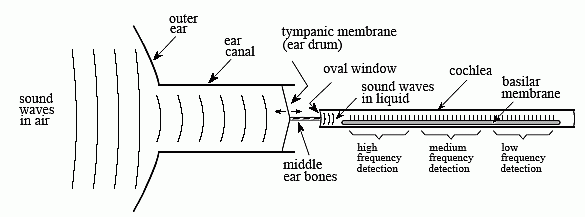
\includegraphics[scale=0.8]{images/human.png}
		\caption{Human Auditary System}
	\end{center}
\end{figure}



Table  below  shows the relationship between sound intensity and perceived loudness. It is common to express sound intensity on a logarithmic scale, called decibel SPL (Sound Power Level). On this scale, zero dB SPL is a sound wave power of $10^{-16} watts/cm2$, about the weakest sound detectable by the human ear. Normal speech is at about 60 dB SPL, while painful damage to the ear occurs at about 140 dB SPL.

\begin{figure}[h]
	\begin{center}
		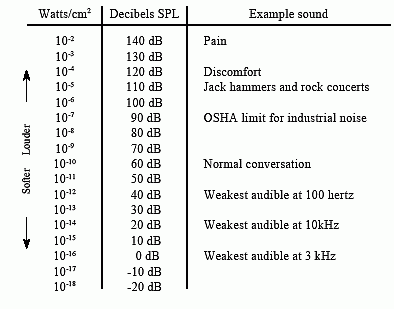
\includegraphics[scale=0.8]{images/intensity.png}
		\caption{Audibility range of sound by human ear at different 
			intensity level}
	\end{center}
\end{figure}

The difference between the loudest and faintest sounds that humans can hear is about 120 dB, a range of one-million in amplitude. Listeners can detect a change in loudness when the signal is altered by about  one dB (a 12 per cent change in amplitude). In other words, there are only about 120 levels of loudness that can be perceived from the faintest whisper to the loudest thunder. The sensitivity of the ear is amazing; when listening to very weak sounds, the ear drum vibrates less than the diameter of a single molecule.
The perception of loudness relates roughly to the sound power to an exponent of 1/3. For example, if you increase the sound power by a factor of ten, listeners will report that the loudness has increased by a factor of about two ($10^{1/3}\approx 2$). This is a major problem for eliminating undesirable environmental sounds, for instance, the beefed-up stereo in the next door apartment. Suppose you diligently cover 99 per cent of your wall with a perfect soundproof material, missing only one per cent of the surface area due to doors, corners, vents, etc. Even though the sound power has been reduced to only 1 per cent of its former value, the perceived loudness has only dropped to about 0.011/3 $\approx$ 0.2, or 20 per cent. 
The range of human hearing is generally considered to be 20 Hz to 20 kHz, but it is far more sensitive to sounds between one kHz and four kHz. For example, listeners can detect sounds as low as 0 dB SPL at three kHz, but require 40 dB SPL at 100 hertz (an amplitude increase of 100). Listeners can tell that two tones are different if their frequencies differ by more than about 0.3 per cent at three kHz. This increases to three percent at 100 hertz. 
The primary advantage of having two ears is the ability to identify the direction of the sound. Human listeners can detect the difference between two sound sources that are placed as little as three degrees apart, about the width of a person at 10 meters. This directional information is obtained in two separate ways. First, frequencies above about one kHz are strongly shadowed by the head. In other words, the ear nearest the sound receives a stronger signal than the ear on the opposite side of the head. The second clue to directionality is that the ear on the far side of the head hears the sound slightly later than the near ear, due to its greater distance from the source. Based on a typical head size (about 22 cm) and the speed of sound (about 340 meters per second), an angular discrimination of three degrees requires a timing precision of about 30 microseconds. Since this timing requires the volley principle, this clue to directionality is predominately used for sounds less than about one kHz. 
Both these sources of directional information are greatly aided by the ability to turn the head and observe the change in the signals. An interesting sensation occurs when a listener is presented with exactly the same sounds to both ears, such as listening to monaural sound through headphones. The brain concludes that the sound is coming from the center of the listener's head.
While human hearing can determine the direction a sound is from, it does poorly in identifying the distance to the sound source. This is because there are few clues available in a sound wave that can provide this information. Human hearing weakly perceives that high frequency sounds are nearby, while low frequency sounds are distant. This is because sound waves dissipate their higher frequencies as they propagate long distances. 







\subsection{Speech Recognition System}
The idea behind speech recognition is to provide a means to
transcribe spoken words into written text. There exist many approaches to achieve this goal. The most simple technique is to build a model for every word that needs to be recognized.Speech signal primarily conveys the words or message being spoken. Area of speech recognition is concerned with determining the underlying meaning in the utterance. Success in speech recognition depends on extracting and modeling the speech dependent characteristics which can effectively distinguish one word from another. The system is a collection of several modules as shown in Figure 2.4.
\begin{figure}
	\begin{center}
		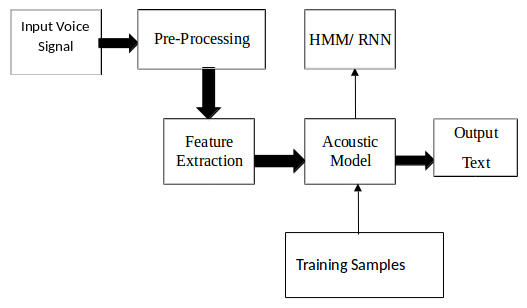
\includegraphics[scale = 0.8]{images/ASR.png}
		\caption{Speech Recognition System}
	\end{center}
\end{figure}

\subsubsection{Input Voice Signal}
The preliminary requirement of the IVR system is the input voice signal from the user such that the system may interact with the user. Most computer systems have the built in microphone facility for this purpose. Also with the help of external microphone the voice signal can be input to the system, the PC sound card produces the equivalent digital representation of received audio. During the phase of training the speech engine the recorded audio is taken and then are used for the sample generation and finally fed into the system model for training purpose and for the interactive voice response system the real time input voice of the system user is taken using the microphone. The circumstances under which input voice signal is uttered plays important role in speech recognition i.e. the factors such as too noisy environment, wrong utterance of word etc may diminish the performance of system. Therefore the input signal must be as clear as possible for the best results possible.

\subsubsection{Preprocessing stage}
The stage of the speech preprocessing refers to the purification of the input voice signal so as to feed it into main speech recognition engine in a suitable format for best outcomes.The preprocessing stage in speech recognition systems is used in order to increase the efficiency of subsequent feature extraction and classification stages and therefore to improve the overall recognition performance. Commonly the preprocessing includes the sampling step, a windowing and a de-noising step as shown in Figure below. At the end of the preprocessing the compressed and filtered speech frames are forwarded to the feature extraction stage.These processes are discussed below in brief.
\begin{figure} [h]
	\begin{center}
		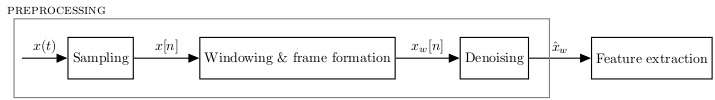
\includegraphics[scale=0.8]{images/prepro.png}
		\caption{Input speech preprocessing}
	\end{center}
\end{figure}

\begin{enumerate}
	\item Sampling stage
	
	
	In order that a computer is able to process the speech signal, it first has to be digitized. Therefore the time-continuous speech signal is sampled and quantized. The result is a time- and value discrete signal. According to the Nyquist-Shannon sampling theorem a time-continuous signal that is band limited to a certain finite frequency fmax needs to be sampled with a sampling frequency of at least $2f_{max}$. In this way it can be reconstructed by its time-discrete signal. Since human speech has a relatively low bandwidth (mostly between 100Hz and 8 KHz) a sampling frequency of 16 KHz is sufficient for speech recognition tasks. 
	
	\item Windowing and frame formation 
	
	
	Speech is a non-stationary time variant signal. We assume that human speech is built from a dictionary of phonemes, while for most of the phonemes the properties of speech remain invariant for a short period of time (~ 5-100ms). In order to obtain frames we multiply the speech signal with a windowing function. This windowing function weights the signal in the time domain and divides it into a sequence of partial signals. By doing so we gain time information of every partial signal keeping in mind that an important step of the preprocessing and feature extraction is a spectral analysis of each frame. 
	\item Denoising stage
	
	
	The stage of denoising or noise reduction, also referred to as enhancing of speech degraded by noise, aims to improve the speech signals quality. The objective is to improve the intelligibility, a measure of how comprehensible speech is. Noise corrupting speech signals can be grouped coarsely into the following three classes: 
	\begin{itemize}
		\item Microphone related noise 
		\item Electrical noise (e.g. electromagnetically induced or radiated noise) and
		\item Environmental noise
	\end{itemize}
	The first two types of noise can be easily compensated by training the speech recognizers on corresponding noisy speech samples, but compensating the environmental noise is not that elementary, due to its high variability. 
	
	Noise is ubiquitous in almost all acoustic environments. The speech signal, that is recorded by a microphone is generally infected by noise originating from various sources. Such contamination can change the characteristics of the speech signals and degrade the speech quality and intelligibility, thereby causing significant harm to human-to-machine communication systems. \\
	Noise detection and reduction for speech applications is often formulated as a digital filtering problem, where the clean speech estimation is obtained by passing the noisy speech through a linear filter. With such a formulation, the core issue of noise reduction becomes how to design an optimal filter that can significantly suppress noise without noticeable speech distortion. 
	
	Noise reduction is the crucial step in speech signal processing. Each signal is contained with some kind of noise in it which deteriotes the speech signal quality. 
	
	Noise reduction techniques depending on the domain of analyses like Time, Frequency or TimeFrequency/Time-Scale. 
	
	The Noise reduction methods are classified into four classes of algorithms: Spectral Subtractive, Subspace, Statistical-model based and Wiener-type. Some popular Noise reduction algorithms are, The log minimum mean square error logMMSE (Ephraim \& Malah 1985), The traditional Wiener (Scalart \& Filho 1996), The spectral subtraction based on reduced-delay convolution (Gustafsson 2001), The exception of the logMMSE-SPU (Cohen \& Berdugo 2002), The logMMSE with speech-presence uncertainty (Cohen Berdugo 2002), The multiband spectral-subtractive (Kamath \& Loizou 2002), The generalized subspace approach (Hu \&Loizou 2003), The perceptually based subspace approach (Jabloun \& Champagne 2003), The Wiener filtering based on wavelet-thresholded multitaper spectra (Hu \& Loizou 2004), Least-Mean-Square (LMS), Adaptive noise cancellation (ANC) [3], Normalized(N) LMS, Modified(M)- NLMS, Error nonlinearity (EN)-LMS, Normalized data nonlinearity (NDN)-LMS adaptation etc. 
	Among those many methods, one of the most simple and effective is the spectral subtraction method. It is quite popular method. Spectral Subtraction method, subtracts the estimated noise from the original signal to enhance the speech recognition. The noise is estimated from the original signal itself and subtracted to the original signal, which thus improves the Signal-to-Noise ratio (SNR). It is assumed that the signal is distorted by a wide-band, stationary, additive noise, the noise estimate is the same during the analysis and the restoration and the phase is the same in the original and restored signal.
	\begin{figure}[h]
		\begin{center}
			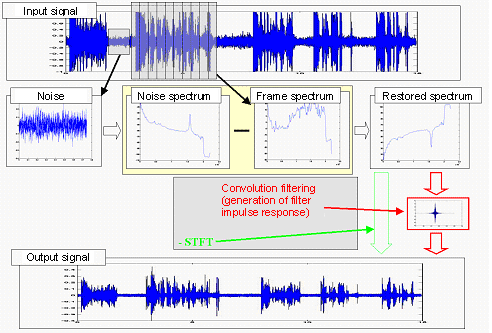
\includegraphics[scale=0.8]{images/image_2.png}
			\caption{Noise Removal Process in input voice signal}
		\end{center}
	\end{figure}
	
\end{enumerate}
\subsubsection{Feature Extraction Stage}
After the preprocessing step, feature extraction is the second component of automatic speech recognition (ASR) systems. It helps to identify the components of audio signals that are good for identifying the linguistic content and discarding all the other stuff such as background noise. The speech signal are slowly timed varying signals (quasi-stationary). When examined over a sufficiently short period of time, the characteristics of signal remain fairly stationary. The information in the speech signal is represented by the short term amplitude of the speech signal.The extraction of feature vectors is based on these short term amplitude spectrum of speech signals. This component should derive descriptive features from the windowed and enhanced speech signal to enable a classification of sounds. The feature extraction is needed because the raw speech signal contains information besides the linguistic message and has a high dimensionality. Both characteristics of the raw speech signal would be unfeasible for the classification of sounds and result in a high word error rate. Therefore, the feature extraction algorithm derives a characteristic feature vector with a lower dimensionality, which is used for the classification of sounds. 


There are several feature extraction techniques such as Linear Predictive Analysis (LPC), Linear Predictive Cepstral Coefficients (LPCC), Mel-Frequency Cepstral Coefficients (MFCC) etc. MFCC is the most commonly used feature extraction method in ASR. To extract a feature vector containing all information about the linguistic message, MFCC mimics the logarithmic perception of loudness and pitch of human auditory system and tries to eliminate speaker dependent characteristics by excluding the fundamental frequency and their harmonics. Among several features generated we consider only the relevant feature set for the classification model. These generated feature set is known as feature vector which define mathematical characteristics of a speech signal. Such feature vectors act as a input to the classification models such as HMM(Hidden Markov Mode)l, RNN(Recurrent Neural Network) etc.\\


\paragraph{Mel Frequency Cepstral Coefficients (MFCC)} \mbox{}


\textbf{Mel Frequency Cepstral Coefficients} is a popular feature extraction technique in speech recognition. The Mel Frequency Cepstral Coefficients are the representation of a windowed short term signal derived from the Fast Fourier Transform (FFT) of the signal on a non linear mel scale of frequency, which is based on the human ear scale.


For the computation of MFCC, the speech signal is divided and framed into 20-40ms long frames. The frames are overlapped for smooth transitions. The next step is to perform Discrete Fourier Transform of the frames. FFT is used to speed up the processing. Then the frequencies obtained from the FFT are wrapped onto the mel scale. A mel is a unit of pitch defined so that pairs of sounds which are perceptually equidistant in pitch are separated by an equal number of mels. The mapping between frequency in Hertz and mel scale is linear below 1000 Hz and logarithmic above 1000 Hz. The mel frequency m can be computed from frequency as 
\begin{equation}
mel(f)=1127ln(1+\frac{f}{700})
\end{equation}

The mel-spaced filterbanks are computed. This is a set of 20-40(standard is 26) triangular filters that we apply to the output of DFT from earlier steps. Then log of the each energy in the filterbank is taken. The next step is to calculate Discrete Cosine Transformation (DCT) which ranges coefficients according to the significance.

\paragraph{Linear Predictive Coding(LPC)} \mbox{}


Linear Predictive Coding (LPC) is a powerful speech analysis technique. The basic idea behind LPC is that a specific speech sample at the current time can be approximated as a linear combination of past speech samples.

Linear Prediction is the technique of computation of a parametric model based on least mean squared error theory. The speech signal is approximated as a linear combination of its precious samples. The obtained LPC coefficients describe the formants. The frequency at which the resonant peaks occur are called the formant frequencies. Thus, in this method, locations of the formants in a speech signal are estimated by computing the linear predictive coefficients over a sliding window and finding the peaks in the spectrum of the resulting LP filer.\\
\paragraph{Perceptual Linear Prediction (PLP)} \mbox{}


The Perceptual Linear Prediction model describes the psychophysics of human hearing process more accurately in feature extraction process. PLP, similar to LPC analysis, is based on the short-term spectrum of speech. But, PLP modifies the short term spectrum of the speech by several psychophysically based transformations to match human auditory system.

The PLP coefficients are calculated by first carrying out N-point DFT. A frequency warping to Bark scale is applied. The critical-band power spectrum is computed through discrete convolution of the power spectrum with the piece-wise approximation of the critical-band curve. The smoothed spectrum is down-sampled at intervals around 1 Bark. The three steps of frequency warping, smoothing and sampling are integrate into a single filter-bank called Bark filter bank. An equal loudness pre-emphasis weight the filter-bank outputs. The equalized values are further processed by Linear Prediction (LP). Applying LP to the warped line spectrum computes the predictor coefficients of a signal that has this warped spectrum as a power spectrum. 

\subsubsection{Acoustic Model}
An acoustic model is used in Automatic Speech Recognition to represent the relationship between an audio signal and the phonemes or other linguistic units that make up speech. The model is learned from a set of audio recordings and their corresponding transcripts. It is created by taking audio recordings of speech, and their text transcriptions, and using software to create statistical representations of the sounds that make up each word.


Acoustic model development is process of developing a speech recognition engine to recognize speech. The software acoustic model breaks the words into the phonemes. There are different popular ways to build this model, some of which are DTW (Dynamic Time Warping), HMM (Hidden Markov Model), RNN (Recurrent Neural Networks) etc.


\paragraph{Hidden Markov Model} \mbox{}\\

A Markov model is a stochastic model which models temporal or sequential data i.e. data that are ordered. It provides a 
way to model the dependencies of current information with previous information. The simplest Markov model is a Markov chain.
Markov Chain models the state of a system with a random variable that changes through time. In this context, the Markov property suggests that the distribution for this variable depends only on the distribution of previous state. 

\begin{minipage}{\linewidth}
	\centering
	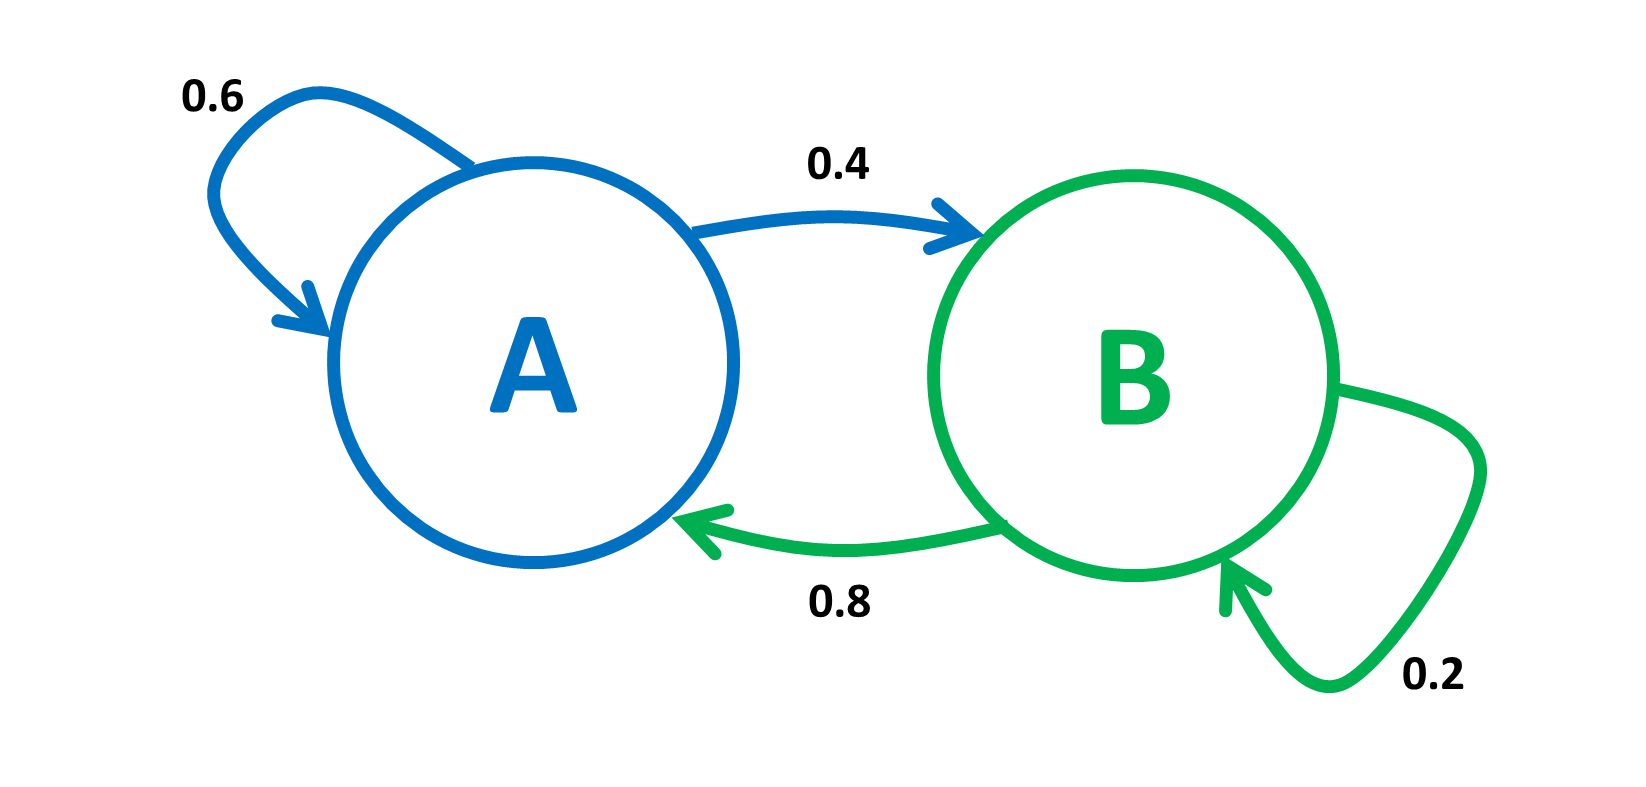
\includegraphics[scale=0.4]{markov-chain} 
	\captionof{figure}{A Markov Chain}
\end{minipage}	

A Hidden Markov Model is a Markov chain for which sate is partially observable. The observations are typically insufficient enough to precisely determine the state. A Hidden Markov Model, is a stochastic model where the states of the model are hidden. Each state can emit an output which is observed.

\begin{minipage}{\linewidth}
	\centering
	
\includegraphics[scale=0.6]{hmm} 
	\captionof{figure}{Structure of a Hidden Markov Model}
\end{minipage}	

\paragraph{Recurrent Neural Network} \mbox{}\\

A recurrent neural network (RNN) is a class of artificial neural network where connections between units form a directed cycle. This allows it to exhibit dynamic temporal behavior.

\begin{minipage}{\linewidth}
	\centering
	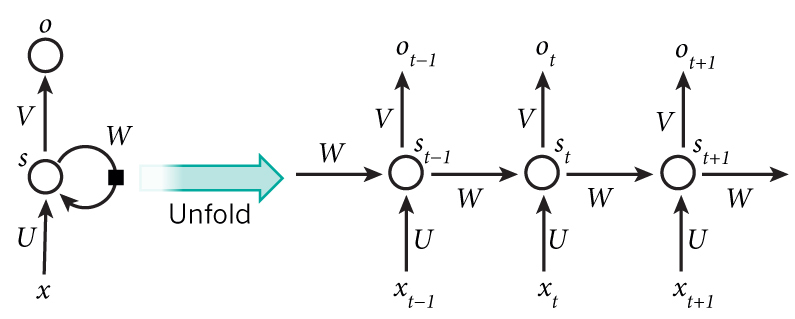
\includegraphics[scale=0.4]{rnn} 
	\captionof{figure}{A recurrent neural network and the unfolding in time}
\end{minipage}	

Recurrent networks, on the other hand, take as their input not just the current input example they see, but also what they perceived one step back in time. The decision a recurrent net reached at time step $t-1$ affects the decision it will reach one moment later at time step $t$. So recurrent networks have two sources of input, the present and the recent past, which combine to determine how they respond to new data, much as we do in life. Recurrent networks are distinguished from feedforward networks by that feedback loop, ingesting their own outputs moment after moment as input. It is often said that recurrent networks have memory. Adding memory to neural networks has a purpose: There is information in the sequence itself, and recurrent nets use it to perform tasks that feedforward networks can not.

The purpose of recurrent nets is to accurately classify sequential input. We rely on the backpropagation of error and gradient descent to do so. Recurrent networks rely on an extension of backpropagation called backpropagation through time, or BPTT. Time, in this case, is simply expressed by a well-defined, ordered series of calculations linking one time step to the next, which is all backpropagation needs to work.

Just as a straight line expresses a change in x alongside a change in y, the gradient expresses the change in all weights with regard to the change in error. If we can not know the gradient, we can not adjust the weights in a direction that will decrease error, and our network ceases to learn. Recurrent nets seeking to establish connections between a final output and events many time steps before were hobbled, because it is very difficult to know how much importance to accord to remote inputs. This is partially because the information flowing through neural nets passes through many stages of multiplication.Because the layers and time steps of deep neural networks relate to each other through multiplication, derivatives are susceptible to vanishing or exploding.

\subparagraph{LSTM RNN :} LSTM stands for Long Short Term Memory. LSTM is a variant of RNN which help preserve the error that can be backpropagated through time and layers. By maintaining a more constant error, they allow recurrent nets to continue to learn over many time steps (over 1000), thereby opening a channel to link causes and effects remotely.

LSTMs contain information outside the normal flow of the recurrent network in a gated cell. Information can be stored in, written to, or read from a cell, much like data in a computer \textquotesingle s memory. The cell makes decisions about what to store, and when to allow reads, writes and erasures, via gates that open and close. Unlike the digital storage on computers, however, these gates are analog, implemented with element-wise multiplication by sigmoids, which are all in the range of 0 to 1.

Those gates act on the signals they receive, and similar to the neural network’s nodes, they block or pass on information based on its strength and import, which they filter with their own sets of weights. Those weights, like the weights that modulate input and hidden states, are adjusted via the recurrent networks learning process. That is, the cells learn when to allow data to enter, leave or be deleted through the iterative process of making guesses, backpropagating error, and adjusting weights via gradient descent.

\begin{minipage}{\linewidth}
	\centering
	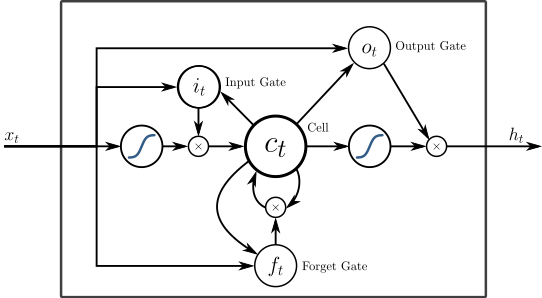
\includegraphics[scale=0.6]{LSTM} 
	\captionof{figure}{A LSTM Block}
\end{minipage}	

\subparagraph{GRU :} GRU stands for Gated Recurrent Unit. A gated recurrent unit (GRU) is basically an LSTM without an output gate, which therefore fully writes the contents from its memory cell to the larger net at each time step.

\begin{minipage}{\linewidth}
	\centering
	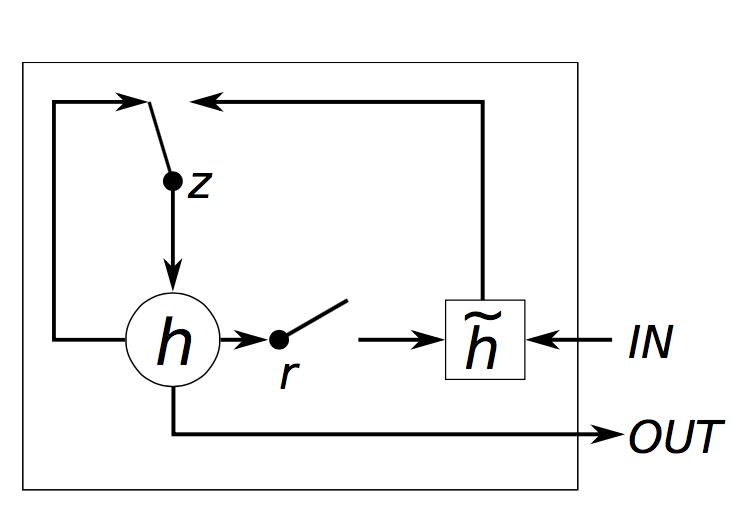
\includegraphics[scale = 0.6]{GRU} 
	\captionof{figure}{A Gated Recurrent Unit Block}
\end{minipage}	

\subsection{Types of ASR system}
Speech Recognition System are characterized by different parameters. Some of the more important of which are discussed here in brief.
\subsubsection{On the basis of input speech signal}
In Speech Recognition System the ability to recognize the speech signal can be subdivided into different classes as below:
\begin{enumerate}
	\item Isolated Words: In this type, system accepts single utterance at a time. And usually requires each utterance to have quiet on both side of sample window and require a speaker to wait between words. Its response will be better for single word but give poor result for multiple words input.
	\item Connected Words: In this type, multiple words given to the system which runs separately as isolated words and having small duration of time between them.
	\item Continuous Speech: In this type, natural speech is spoken by the user that is detectable by the machine. Continuous speech recognition is difficult to create because they utilize special method for implementation.
	\item Spontaneous Speech: In this type natural and spontaneous word has the ability to handle a variety of natural features such as words run together including mispronunciations, non-words and false statements, which are difficult to read.
\end{enumerate}
\subsubsection{On the basis of speaker model}
Every speaker has unique properties which affects the voice. On the basis of these properties system is divided into two main classes.
\begin{enumerate}
	\item Speaker Dependent Model:Speaker dependent model depends on specific speaker. These models are easier to implement and less expensive. It gives more accurate result for specific speaker and less accurate result for other speakers
	\item Speaker Independent Model:Speaker independent models depend upon many speakers. These models are difficult to implement and more expensive. It gives more accurate result for many speakers and less accurate result for specific speaker.
\end{enumerate}

\subsubsection{On the basis of type of vocabulary}
\begin{enumerate}
	\item Small size vocabulary that includes tens of words. 
	\item Medium size vocabulary that includes hundreds of words. 
	\item Large vocabulary size that includes thousands of words. 
	\item Very large size vocabulary that includes tens of thousands of words.
	\item Out of size vocabulary includes mapping a word from the vocabulary into the unknown word.
	
\end{enumerate}

\subsection{Interactive Voice Response System}

The Interactive Voice Recognition (IVR) systems through speech recognition is now enabling to go beyond the touch-tone interface models. In an IVR system, an automated message or greeting is played by the system to the caller/user. The user then responds the automated message with particular speech (voice) which is when processed through the speech processing system, outputs the corresponding speech in the text format. Now, the generated text is to be processed to make the system choose the reasonable next message or sequence of task to be followed. Then, the system selects the message (text or recorded speech) and again outputs the selected speech message back to the caller/user. This process continues on until the user/caller is transferred to a human agent or the connection is terminated. 

A system is needed on the receiving end to perform all these automated tasks. The system implements following steps to make a specific Interactive voice response system
in order to carry out its task as per the command from the user given to the system: 

\subsubsection{SoftPhone}
Softphone is basically just a part of the system which has same functions as an ordinary telephones. The IVR should be able to receive calls coming from other telephones/devices. It just handles the incoming calls. 
\subsubsection{Call Handler}
Then, a call handler is used to manage those incoming calls. This presents the caller with the auto generated voice greeting message through the speaker which then offers the selectable menu items. The caller responds to that menu through speech. 
Call handler is actually, a super set to the speech recognition system which carries out entire task of converting speech to the text. 

After the text is generated, it should be able to process the text into equivalent operations. For that the system, takes thus converted text as input and performs a search throughout the database and selects a match. During selection of a match, there arises three different cases:
\begin{itemize}
	\item Call forwarding/transferring
	
	User/Caller may ask to transfer the call to any human agent. 
	\item Automated Response Reply 
	
	
	The user might have certain queries to the system which is in the knowledge base of the system. 
	
	\item Call Termination 
	
	
	User/Caller may terminate the call after finishing their queries. 
	
	
	
	Now, in the case of the response reply, the system has to convert the selected text message back to the speech which is done by the text-to-speech module of the system and reply back to the user/caller. 
\end{itemize}







\newpage

\section{METHODOLOGY}


\subsection{Methodology overview}

\begin{figure}[h]
	\begin{center}
		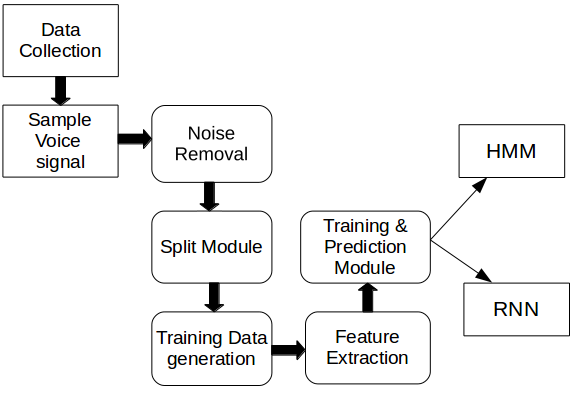
\includegraphics[scale=0.8]{images/methodology.png}
		\caption{Outline of the project methodology }
		\label{methodology}
	\end{center}
\end{figure}

Before beginning the project work we went through several researches. Through the researches we learnt about several useful methodologies so that we can approach towards the project development phase. Going through several papers and books we selected suitable approach that fulfilled our needs as per our domain system. Figure 3.1 shows the block diagram that represents the overall outline of the project development methodology. The preliminary stage began with the collection of sample voice signal from different speakers using recording software tool called audacity. The recorded voice signal consist of external noises which were depreciated using the noice removal technique. After that from each recorded signals training data samples were generated using split module which makes the data samples suitable for feature extraction. Using those samples specific feature extraction technique is used to extract unique feature vectors. In our case we used MFCC for feature extraction purpose. The extractd features were used to train the prediction model. In our project we have used two approaches for prediction purpose which are HMM and RNN approaches respectively. The details regarding the methodology is discussed in the sections below.



\subsection{Data Collection}
For a project data is the most important part that may be of various forms such as text, audio, video etc. In our case we required the audio data
as it deals with the recognition of voice from the user to interact with 
system.Thus large samples of data are required for the training of the 
model and hence enhance the performance ability of the recognition model.
The Data collection phase is the initial phase of the project to 
begin with. This stage has been divided to two phases as discussed below:

\subsubsection{Sample Voice Collection}
In collecting required data for the project we needed the Nepali spoken 
words as we were dealing for the interactive voice response system
using Nepali speech. The sources for Nepali speech data were not available
in the web so that we had to manually collect the data from the individuals
The sample voice collection was done from several individual possible.
\begin{figure}[h]
	\begin{center}
		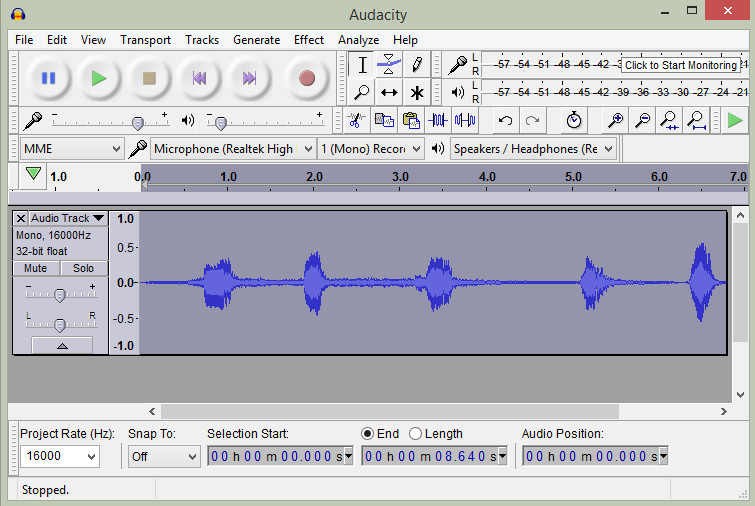
\includegraphics[scale=0.7]{images/audacity.png}
		\caption{Audacity Interface for sound sample recording}
		\label{audacity}
	\end{center}
\end{figure}


For recording purpose we used a simple software called "Audacity", which
is free and cross platform software Licensed under the GNU General Public License (GPL).
It easily runs on several platforms such as Windows, Mac OS X/mac OS and GNU/Linux.
Audacity can record live audio through a microphone or mixer, 
or digitize recordings from other media. With some sound cards, and on 
any recent version of Windows, Audacity can also capture streaming audio. 
Thus for collecting sound samples we developed a simple tutorial on
recording the speech and collected data from several individuals and also manually 
recorded the voices.As our Devanagari script is very vast for the preliminary stage 
we are working with the simple sound samples from numbers 0 to 9. For our
project we used the sound samples of  frequency rate of 16000Hz recorded using
the mono-channel configuration.Similarly we used 16-bit samples for the project.
The sample voice collected thus were used for the training data generation.



\subsubsection{Training Data Generation}
After collecting the sample voices from multiple sources, we need to create training samples to be used in speech recognition. The sample voice contains speech signals numbered from $0 - 9$. Now these samples need to be separated into individual files each containing a digit so that it can be used as training samples. 

To generate sample of each digit, we have to detect silence zones from the sample file and separate each based on those silence regions.

Now, to detect the silence zones, it \textquotesingle  s highly depended on the audio signal. We need to detect the threshold level, below which the sound can be considered as silent. In order to detect the threshold level, first we fragment the whole audio sample into certain number of frames based on sample width. Then, we calculate the root mean square value which gives an approximate estimate of threshold level, below which the sound frames can be considered silence and above it as voiced activity.

After the detection of threshold level, we need to partition the sound sample. Based on the threshold level for a sound sample, now we detect the silent zones, and thereafter the ranges. We define a minimum silence length in second. And the audio sample is fragmented into number of sample per frame based on silence length. If a frame \textquotesingle s rms value is less than threshold then, the frame is considered as silent frame, and so on silent ranges are determined. These ranges can be complimented then to generate the ranges that actually contains the voice. Then the audio sample is partitioned based on these non-silence activity ranges.
\begin{figure}[h]
	\begin{center}
		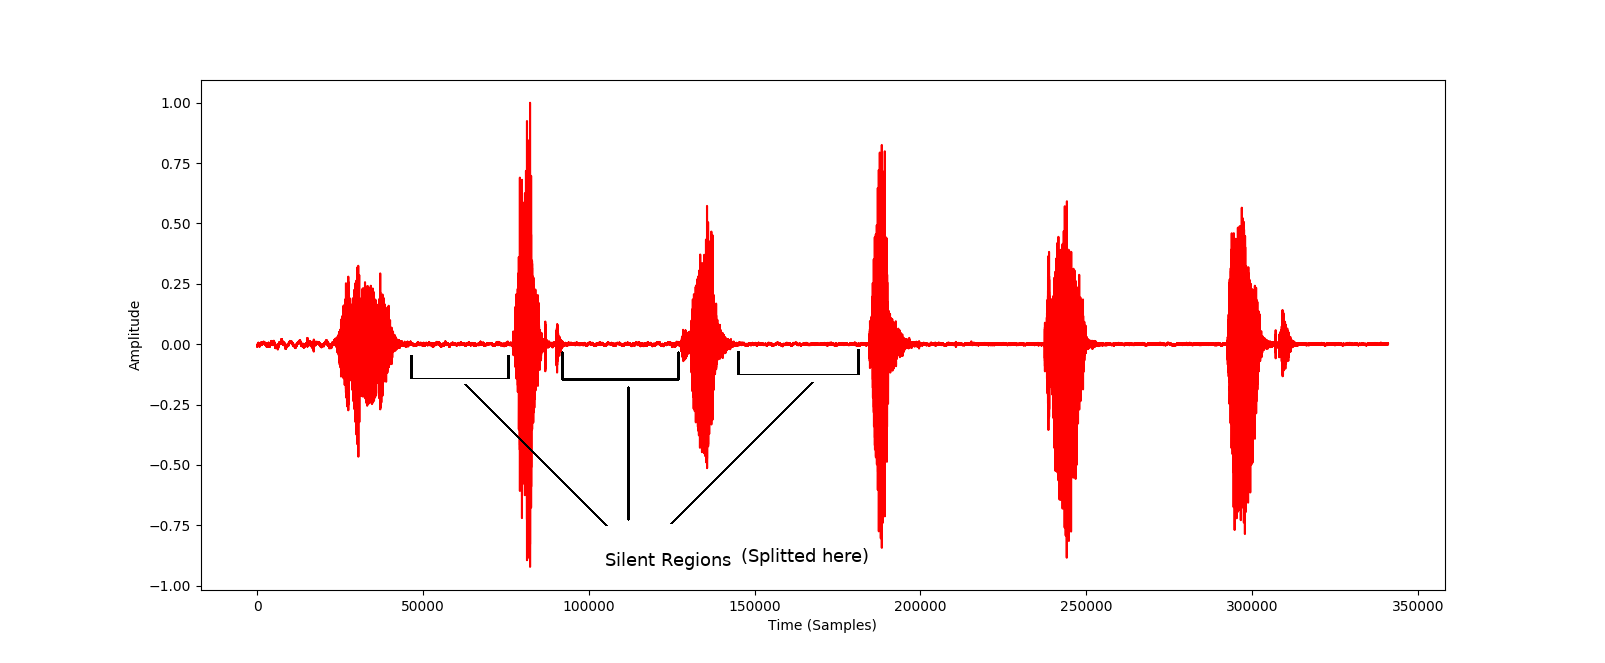
\includegraphics[width=6in]{images/sample.png}
		\caption{Training samples generation from recorded voice}
		\label{sample}
	\end{center}
\end{figure}

\subsection{Noise Reduction}

The speech signal may contain some noise. Actually, most of the speech signals contains background noise. This noise degrades the quality of the speech signal and create hindrance in the processing the speech. Thus, a noise reduction algorithm is needed to reduce the noise level without affecting the speech signal quality. One of the noise reduction algorithm used in this project is Spectral Subtraction method. It is performed independently in the frequency bands corresponding to the auditory critical bands.

The spectral subtraction method is a simple and effective method of noise reduction. In this method, an average signal spectrum and average noise spectrum are estimated in parts of the recording and subtracted from each other, so that average signal-to-noise ratio (SNR) is improved. It is assumed that the signal is distorted by a wide-band, stationary, additive noise, the noise estimate is the same during the analysis and the restoration and the phase is the same in the original and restored signal.

The noisy signal y(m) is a sum of the desired signal x(m) and the noise n(m):
\begin{equation}
y(m) = x(m) + n(m)
\end{equation}

In the frequency domain, this may be denoted as:
\begin{equation}
Y(j\omega) = X(j\omega) + N(j\omega) \Rightarrow X(j\omega) = Y(j\omega) – N(j\omega)\\
\end{equation}
where $Y(j\omega), X(j\omega), N(j\omega)$ are Fourier transforms of y(m), x(m), n(m), respectively.
To take the Discrete Fourier Transform of the frame, perform the following:
\begin{equation}
Y_i(k) =
\sum_{m=1}^{N}
y_i(m)h(m)e^{-j2\pi km/N} \qquad 1\leq k\leq K\\
\end{equation}

where $h(m)$ is an N sample long analysis window (e.g. hamming window), and K is the length of the DFT. The magnitude spectrum for the speech frame $y_i(m)$ is given by:

\begin{equation}
M_{i}(k) = | Y_{i}(k) |
\end{equation}

The phase spectrum is calculated in the following way:
\begin{equation}
\theta_i(k) = tan^{-1}(\frac{Im(Y_i(k))}{Re(Y_i(k))}) \\
\end{equation}


The statistic parameters of the noise are not known, thus the noise and the speech signal are replaced by their estimates:

\begin{equation}
\hat{X}(j\omega) = Y(j\omega) - \hat{N}(j\omega)\\
\end{equation}

Noise is the time-average estimate of first few frames of the speech signal.
\begin{equation}
\hat{N}(j\omega) = \frac{1}{K}  \sum_{i=0}^{K-1}|N_i(j\omega)| \\
\end{equation}

The noise reduced clean speech signal is then obtained by performing the inverse Fourier transform of $X(j\omega)$
\begin{figure}[h]
	\begin{center}
		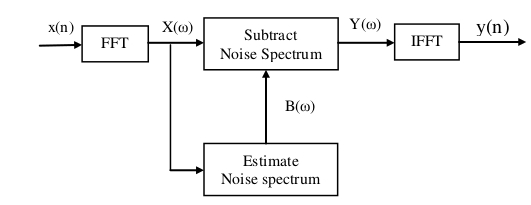
\includegraphics[width=6in]{images/noise.png}
		\caption{Noise removal process in speech signal}
		\label{noise}
	\end{center}
\end{figure}


The procedural Explanation of the noise removal technique of the input speech signal is discussed below:

The basic principle is as follows: if we assume additive noise, then we can subtract the noise spectrum from the noisy speech spectrum, so we are left with what should look like the clean speech spectrum. For this we need to know what the noise spectrum looks like, so we estimate it during regions of no speech (parts of the signal that contain only noise) and then assume it won't change much from frame to frame.

Let's assume a clean time domain signal, $x(m)$ to which we add additive noise, $n(m)$.The signal we actually see is the sum $y(m) = x(m) + n(m)$. We wish to estimate the true value of $x(m)$ given $y(m)$ only.

The first step in spectral subtraction is to frame the speech signal into short, overlapping frames. Typically frames are taken to be about 20ms long. For a 16KHz sampled audio file, this corresponds to $$0.020s * 16,000 samples/s = 320\enspace samples$$ We then use an overlap of 50\%, or about 200 samples. This means the first frame starts at sample 0, the second starts at sample 200, the third at 400 etc.

Then, we need a window, which contains certain number of frames. We used Hamming window for this project. We then take the discrete Fourier transform of each frame and extract the magnitude and phase spectrum from each. Let $y_i(m)$ be framed time domain signal and $Y_i(k)$ is its complex Discrete Fourier Transform, (DFT) where m ranges over 1-400 (if our frames are 400 samples ) and $i$,  ranges over the number of frames. Then $M_i(k)$ is the magnitude spectrum of frame $i$.

We used Fast Fourier Transform (FFT) in real world practice.
The magnitude spectrum for the speech frame $y_i(m)$ is given by:
\begin{equation}
M_i(k) = |(Y_i(k)|
\end{equation}


\vspace{9mm}
\begin{lstlisting}
Pseudocode
windowed_frame = frame .* hamming(length(frame));
complex_spec = fft(windowed_frame,512); 
mag_spec = abs(complex_spec);
phase_spec = angle(complex_spec);
\end{lstlisting}


Now, to get the estimate of noise, a common assumption is that the first few frames of an audio signal consist of silence.To get our noise estimate, we can take the mean of the first few or so frames. With the magnitude and noise estimate for each frame, now we proceed with spectral subtraction: subtraction of noise estimate. It can be done as:
\begin{equation}
\hat{M}_i(k) =
\begin{cases}
	M_i(k) - N_i(k)\qquad if\enspace M_i(k) \geq N_i(k)\\
	0 \hspace{3cm} if\enspace M_i(k) < N_i(k)\\
\end{cases}
\end{equation}


Here, $\hat{M}_i(k)$ is the estimated clean spectrum. $M_i(k)$ is the noisy spectrum. And $N_i(k)$ is the noise estimate.

Note that we restrict our estimated magnitude spectrum to be positive, since magnitude spectrum must be.

\begin{lstlisting}
clean_spec = mag_spec - noise_est;
clean_spec(clean_spec < 0) = 0;
\end{lstlisting}

Now we have an estimate of the clean spectrum for every frame. With this, we would like to reconstruct the original audio recording which will  have less background noise. For this we use the clean spectrum $M_i(k)$ and phase spectrum from each frame that we calculated at the beginning.

Then, the estimated clean complex spectrum for each frame $Y_i(k)$ (enh\_spec) is


\begin{lstlisting}
enh_spec = clean_spec.*exp(j*phase_spec)

\end{lstlisting}



Now, Inverse FFT (IFFT) of $\hat{Y}_i(k)$ is calculated to reconstruct our original signal $\hat{x}(m)$ and do overlap add of the resulting time-domain frames.



\subsection{Feature Extraction}
The goal of feature extraction is to transform the input waveform into a sequence of \textbf{feature vectors}, each vector representing the information in a small time window of the signal. The most commonly used feature extraction is the \textbf{MFCC, the Mel Frequency Cepstral Coefficients}. These are based on the important idea of cepstrum. The steps in MFCC are shown in Fig 3.4 and described in following sections. 

\begin{figure}[h]
	\begin{center}
		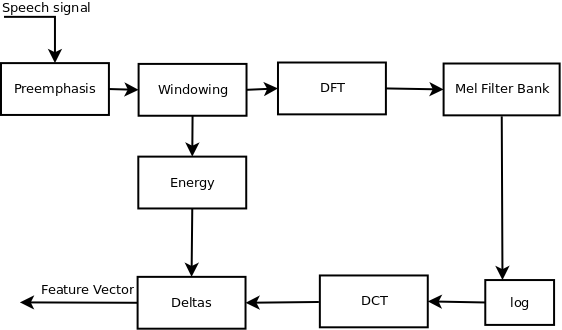
\includegraphics[scale=0.3]{images/feature-blockdiagram.png}
		\caption{Stages in feature extraction}
		\label{feature}
	\end{center}
\end{figure}

\subsubsection{Preemphasis}
The first stage in MFCC feature extraction is to boost the amount of energy in the high frequencies. The spectrum of voiced segments for vowels shows that there is more energy at the lower frequencies than the higher frequencies. This drop in energy across frequencies is called spectral tilt and is caused by the nature of the glottal pulse. Boosting the high frequency energy makes information from these higher formants more available to the acoustic model.
\begin{figure}[h]
	\centerline{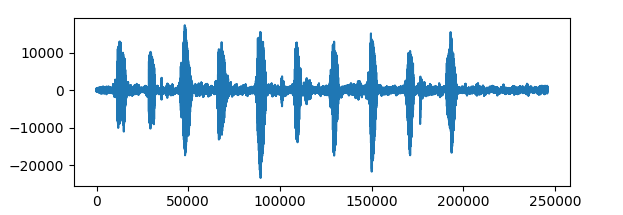
\includegraphics[scale=0.50]{images/beforepreemphasis.png}}
	\caption{Speech signal before pre-emphasis}
\end{figure}

\begin{figure}[h]
	\centerline{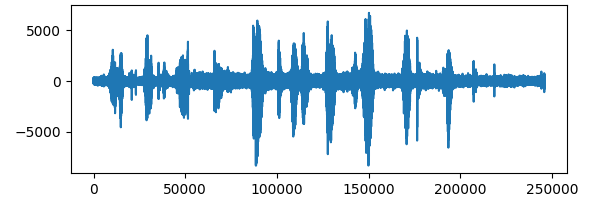
\includegraphics[scale=0.50]{images/afterpreemphasis.png}}
	\caption{Speech signal after pre-emphasis}
\end{figure}

\subsubsection{Windowing}
Speech signal are non-stationary signals, meaning that their statistical properties are not constant across time. So, we take spectral features from a small window of speech signal so that we can make an assumption that the signal is stationary (i.e. the statistical properties are constant within the region).The extraction of the signal takes place by multiplying the value of the signal at the time n, \textit{s[n]}, with the value of the window at time n, \textit{w[n]}:
\begin{equation}
y[n] = w[n]s[n]
\end{equation}

We can characterize the windowing process by three parameters : how \textbf{wide} is the window, what is the \textbf{offset} between the successive windows and what is the \textbf{shape} of the window.
We call the speech extracted  from each window a \textbf{frame}, the number of milliseconds in the frame the \textbf{frame size} and the number of milliseconds between the left edges of the successive windows the \textbf{frames shift step}.

The signals are framed into 20-40ms. We have used frames of frame size 25ms. So, for a signal with 16 KHz signal, we have 0.025*16000 = 400 samples. The frame step is taken as 10ms i.e. 160 samples. This allows for overlapping of the frames. The first 400 samples start at sample 0, the next starting at sample 160, etc. until end of the signal is reached.

\subsubsection{Discrete Fourier Transform}
The next step to extract information from the frames; we need to know how much energy the signal contains at different frequency bands. For this, we use Discrete Fourier Transform (DFT).

The input to the DFT is a windowed signal \textit{x[n]...x[m]}. To take the DFT of the frame, we perform the following:
\begin{equation}
S_i(k) = \sum_{n=1}^{N}s_i(n)h(n)e^{\frac{-j2 \pi kn}{N}}\quad\quad  1\leq k\leq K 
\end{equation}


where h(n) is an N sample long analysis window and K is the length of the DFT.


The peridiogram-based power spectral estimate for the frame $s_i$(n) is given by
\begin{equation}
P_i(k) = \frac{1}{N}|S_i(k)^2 
\end{equation}

\subsubsection{Mel Filter Bank}
The results of FFT will be amount of energy at each frequency band. Human hearing, however, is not equally sensitive at all frequency bands. It is less sensitive at higher frequencies, roughly above 1000 Hz. The modelling of this human hearing property during feature extraction improves speech recognition performance. The form of the model used in MFCCs is to warp the frequencies output of the FFT onto the mel scale. A \textbf{mel} is a unit of pitch defined so that the pairs of sounds perceptually equidistant in pitch are separated by an equal number of mels. The mapping between frequency in Hz and the mel scale is linear below 1000 Hz and logarithmic above 1000 Hz. The mel frequency m can be computed from frequency as 
\begin{equation}
mel(f)=1127ln(1+\frac{f}{700})
\end{equation}
The filter bank is a set of 20-40 (26 is standard) triangular filters applied to the periodogram power spectral estimate. For 26 filters, we get 26 vectors. The Mel-spaced filterbanks can be computed from the following equations


\begin{equation}
	H_m(k) =
	\begin{cases}
		0 & k<f(m-1) \\
		\frac{k - f(m-1)}{f(m) - f(m-1)} & f(m-1) \leq k \leq f(m) \\
		1 & k = f(m)\\
		\frac{f(m+1) - k }{f(m+1) - f(m)} & f(m) \leq k \leq f(m+1) \\
		0 & k>f(m+1)
	\end{cases}
\end{equation}

where M is the number of filter we want.    
To calculate the filterbank energies, each filterbank is multiplies with the power spectrum, then added up. This provides the energy in each filterbanks.


Finally, we take the log of each of the mel spectrum values. In general, the human response to the signal level is logarithmic; human are less sensitive to slight differences in amplitude at high amplitudes than at low amplitudes. In addition, using a log makes the feature estimates less sensitive to variations in input.
\begin{figure}[h]
	\centerline{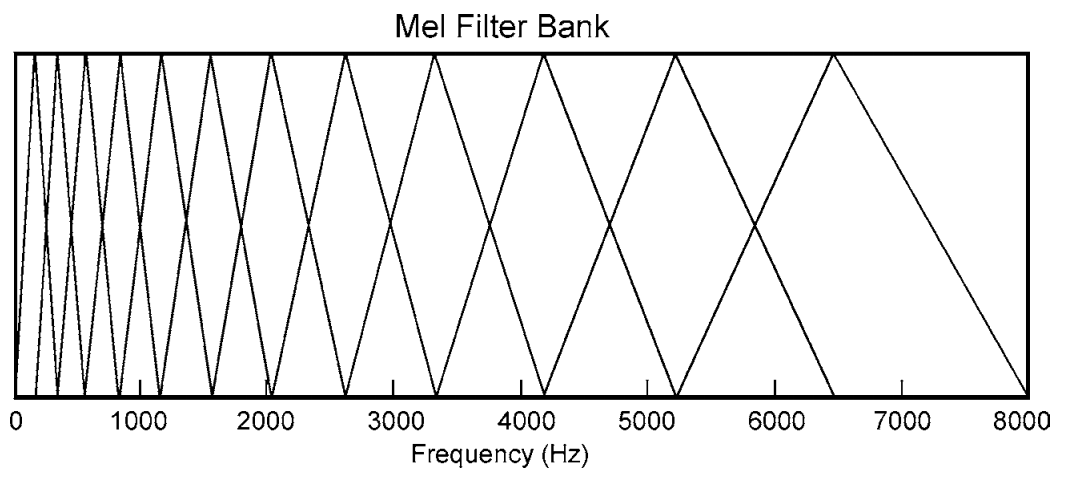
\includegraphics[scale=0.35]{images/filterbanks.png}}
	\caption{Mel filter Bank}
\end{figure}


\subsubsection{Discrete Cosine Transform}
The final step is to compute Discrete Cosine Transform (DCT) of the log filterbank energies. The filterbank energies are quite correlated with each other as our filterbanks are overlapping. The DCT decorrelates the filter bank coefficients and yield a compressed representation of the filter banks.

\subsubsection{Deltas and Energy}
The extraction of the cepstrum via DCT results in cepstral coefficients for each frame. The energy within a frame is also an important feature that can added to the cepstral coefficients. We usually add the the log energy to the cepstral coefficients.


We also can add a delta or velocity feature to the cepstral coefficients for better performance. The delta features represents the change between frames in the corresponding cepstral/energy features. The deltas can be computed from the difference between frames; thus the delta value \textit{d(t)} for a particular cepstral value \textit{c(t)} for time \textit{t} can be estimated as
\begin{equation}
d(t) = \frac{\sum_{n=1}^{N}n(c(t+n) - c(t-n))}{2 \sum_{n=1}^{N}n^2}
\end{equation}


\subsection{Prediction}

Prediction refers to predicting the sound samples based on the Features Extracted. Prediction is done first by teaching a model from the data sets that we have and then making it to predict for new inputs. The Speech Recognition for IVR system is an Isolated Word Recognizer problem. The MFCC features obtained from above for each time frames act as the data sources that can be feed to train the model and later on predict from the model. Prediction is done by using Hidden Markov Models and Recurrent Neural Networks. These both are different approaches but with both approaches implied we can compare both and select the best one.


\subsubsection{Hidden Markov Model}


A hidden Markov model is defined as a pair of stochastic processes ($X$,$Y$). The $X$ process is
a first order Markov chain, and is not directly observable, while the $Y$ process is a sequence
of random variables taking values in the space of acoustic parameters, or observations.

Let $y$ $\epsilon$  $Y$ be a variable representing observations and $i$ , $j$ $\epsilon$  $X$ be a variable representing model states, the model can be represented by following parameters

\[ A = \{a _{i,j} | i,j \epsilon X \} \hspace{1cm}   Transition Probabilities \]
\[ B = \{b _{i,j} | i,j \epsilon X \} \hspace{1cm}   Output Distributions \]
\[  \Pi  = \{\pi _{i} | i \epsilon X \}  \hspace{1cm}  Initial Probabilites \]


with the following definitions:

\begin{equation} a _{i,j} = P(X _{t} = j | X _{t-1} = i ) \end{equation}
\begin{equation} b _{i,j}(y) = P(Y _{t} = y | X _{t-1} = i ,  X _{t} = j ) \end{equation}
\begin{equation} \pi _{i} = p(X _{0} = i) \end{equation}

For convenience, the HMM is generally represented in a complex notation
\begin{equation} \lambda = (A,B, \Pi ) \end{equation}

\paragraph{Evaluation} \mbox{}\\
Evaluation in HMM refers to efficiently computing $ P(O|\lambda) $, the probability of the observation sequence, given the observation sequence $ O = (0 _{1}, 0 _{2},0 _{3},...,0 _{n}) $ and an HMM model $ \lambda = (A,B, \Pi ) $. This can be solved by using either Forward or Backward Procedure.
\subparagraph{The Forward Procedure:}
One way to calculate $ P(O|\lambda) $ given $ \lambda $ is to enumerate all possible combinations. Considering that there are N total observable symbols at each state and we
wish to calculate the probability of observation sequence $ O = (o _{1}, o _{2},o _{3},...,o _{n}) $, There will be $ N^{T} $ state sequences. And, calculating the probability for each such sequence would require $(2T -1)$ multiplications and in total we would require $(2T -1) * N^{T} $ multiplications and $ N^{T} $ additions.This is inefficient and a more efficient algorithm is required. Forward algorithm is
an efficient algorithm for this. Consider the forward variable: 

\begin{equation} \alpha _{t} (i) = P(o _{1}, o _{2},o _{3},...,o _{t},q(t) = i|\lambda)  \end{equation}

that is the probability of the partial observation sequence, $o _{1}, o _{2},o _{3},...,o _{t}$ (until time t) and
state $i$ at time $t$, given the model $\lambda$. We can solve for $\alpha _{t} (i)$ inductively as follow.
\begin{enumerate}
	\item Initialization 
	\begin{equation} \alpha_{1}(i) = \Pi_{i}b_{i}(o_{i}), 1 \leq i \leq N  \end{equation}
	
	\item Induction
	\begin{equation} \alpha_{t+1}(j) = \{ \sum_{i=1}^{N}\alpha_{t}(i)a(i,j) \} b_{j}(i)(o_{t+1}) ,1 \leq t \leq T-1 ; 1 \leq j \leq N \end{equation}
	
	\item Termination
	\begin{equation} P(O|\lambda) = \sum_{i=1}^{N} \alpha_{T}(i) \end{equation}
\end{enumerate}

\subparagraph{The Backward Procedure:}
In a similar manner, we can consider a backward variable $ \beta_{t}(i) $ defined as 

\begin{equation} \beta _{t} (i) = P(o _{t+1}, o _{t+2},o _{t+3},...,o _{T},q(t) = i|\lambda)  \end{equation}

that is the probability of the partial observation of sequence from t+1 to end, given state $i$ at time $t$ and the model $\lambda$. We can solve for $\beta _{t} (i)$ inductively as follow.
\begin{enumerate}
	\item Initialization 
	\begin{equation} \beta_{T}(i) = 1, 1 \leq i \leq N  \end{equation}
	
	\item Induction
	\begin{equation} \beta_{t}(i) =  \sum_{j=1}^{N}a(ij) b_{j}(o_{t+1})\beta_{t+1}(j) , t = T-1, T-2, ... , 1  and  1 \leq i \leq N \end{equation}
	
\end{enumerate}

\paragraph{Decoding} \mbox{}\\
Decoding refers to finding or choosing  a state sequence $ Q = (q_{1},q_{2},q_{3},...,q_{n}) $ that best explains the observation sequence $ O = (o_{1},o_{2},o_{3},...,o_{n}) $ for an HMM model $ \lambda = (A,B, \Pi ) $. This problem can be solved by using the Forward-Backward algorithm too but the Viterbi algorithm is the most widely used solution to this "Optimal State" problem. To find the state sequence $ Q = (q_{1},q_{2},q_{3},...,q_{n}) $ for the observation sequence $ O = (o_{1},o_{2},o_{3},...,o_{n}) $ , We need to define the quantity :
\begin{equation} \delta_{t}(i) = max(q_{1},q_{2},q_{3},...,q_{t-1})P(q_{1},q_{2},q_{3},...,q_{t-1},q_{t}=o_{1},o_{2},o_{3},...,o_{t}) | \lambda \end{equation}
This is, $\lambda_{t}(i)$ is the best source along a single path, at time t, which
accounts for the first $t$ observations and ends in state $i$. By induction, we have
\begin{equation} \delta_{t+1}(j) = max(i)[\delta_{t+1}(j)a(ij)]b_{j}(o_{t+1}) \end{equation}

To actually retrieve the state sequence we need to keep track of the arguments that
maximized the above equation, for each $t$ and $j$. We do this via the array $\Psi_{t}(j)$.The complete
procedure for finding the best state sequence can now be stated as follow.

\begin{enumerate}
	\item Initialization
	\begin{equation} \delta_{t}(i) = \Pi_{i}b_{i}(o_{t}) , 1 \leq i \leq N \end{equation}
	\begin{equation} \Psi_{1}(j) = 0 \end{equation}
	
	\item Recursion
	\begin{equation} \delta_{t}(i) = max(1 \leq i \leq N)[\delta_{t-1}(i)a(ij)]b_{j}(o_{t}), 1 \leq j \leq N , 1 \leq t \leq T \end{equation}
	\begin{equation} \Psi_{t}(j) = argmax(1 \leq i \leq N)\delta_{t-1}(i)a(ij), 1 \leq j \leq N , 1 \leq t \leq T \end{equation}
	
	\item Termination
	\begin{equation} P = max(1 \leq i \leq N) [\delta_{T}(i)] \end{equation}
	\begin{equation} q_{T} = argmax(1 \leq i \leq N) [\delta_{T}(i)] \end{equation}
	
	\item Backtracking
	\begin{equation} q_{t} = \Psi_{t+1}(q_{t+1}), t = T-1, T-2,...,1 \end{equation}
\end{enumerate}
The above algorithms are implemented in log scale because of low values of probability.
Also, it is worth noting that viterbi algorithm is similar to forward implementation of the
forward procedure except some subtle differences.

\paragraph{Learning} \mbox{}\\

Learning refers to adjusting the model parameters $ \lambda = (A,B, \Pi ) $ to maximize $ P(O|\delta)$. This is the most difficult problem of HMMs. The algorithm used for this step is the buam-welch algorithm. Baum-Welch re-estimation uses EM (Expected maximization) to determine the HMM parameters.

\begin{enumerate}
	\item Define $\xi(i,j)$ as probability of being in state $i$ at time $t$, and in state $j$ at time $t+1$
	
	\[ \xi(i,j) = \frac{\alpha_{t}(i)a_{ij}b_{j}(O_{t+1})\beta_{t+1}(j)}{P(O|\lambda)} \]
	
	\begin{equation} = \frac{\alpha_{t}(i)a_{ij}b_{j}(O_{t+1})\beta_{t+1}(j)}{\sum_{i=1}^{N} \sum_{j=1}^{N} \alpha_{t}(i)a_{ij}b_{j}(O_{t+1})\beta_{t+1}(j)}  \end{equation}
	
	\item Define $\gamma_{t}(i)$ as the probability off being in state $i$ at time $t$, given the observation sequence.
	
	\begin{equation}
	\gamma_{t}(i) = \sum_{j=1}^{N} \xi(i,j) \end{equation}
	
	\item So, $\sum_{t=1}^{T} \gamma_{t}(i)$ is the expected number of times state $i$ is visited, and $\sum_{t=1}^{T-1}\xi_{t}(i,j)$ is the expected number of transitions from state i to state j.
	
	\item Now the parameters of HMM are updated as \\
	$\Pi_{i} = $ Expected frequency in state $i$ at time $t = 1 = \gamma_{1}(i)$\\
	$a_{ij} = $ (expected number of transition from state i to state j) / (expected number of transition from state i) :
	
	\begin{equation} a_{ij} = \frac{\sum \xi_{t}(i,j)}{\sum \gamma_{t}(i)} \end{equation}
	$b_{j}(k) = $ (expected number of times in state j and observing symbol k) / (expected number of times in state j):
	
	\begin{equation} b_{j}(k) = \frac{\sum_{t,ot=k} \gamma_{t}(j)}{\sum_{t}\xi(j)} \end{equation}
\end{enumerate}

Continuous observation densities in HMMs When introducing HMM, we defined the observations of the HMMs to be discrete symbols from a finite alphabet, and therefore we could use a discrete probability density within each state of this model. These are called discrete HMMs. The problem with this approach is that the observations are often continuous in most of the practical applications. Although it is possible to convert such continuous signal representations into a sequence of discrete symbols via vector quantization codebooks etc, there might be serious degradation associated with such discretization of the continuous signal. Hence, it would be advantageous to be able to use HMMs with continuous observation densities to model continuous signal representations directly.

To use continuous observation density, some restrictions must be placed on the form of the model probability density function (pdf) to ensure that the parameters of the pdf can be re-estimated in a consistent way. The most general representation of the pdf, for which a re-estimation procedure has been formulated, is a finite mixture of the form
\begin{equation} b_{j}(o) = \sum_{k=1}^{M}C(jk)N[O,\mu_{jk},U_{jk}] , 1 \leq j \leq N \end{equation}

Where $O$ is the observation vector being modeled. $c_{jk}$ is the mixture coefficient for the $kj^{th}$ mixture in the state $j$ and $N$ is any log-concave or elliptically symmetric density. The mostly used distribution is the Gaussian distribution. The equations of a multivariate gaussian distribution for independent random variables is where $\mu_{j}$ is the mean vector, and
the covariance matrix $U_{jk}$ reduces to $\sigma_{ii}$ , the product

\begin{equation} f(X=x|\mu,\textstyle \sum) = \prod_{i=1}^{N} \frac{1}{(2\pi)^{\frac{1}{2}}} exp {- \frac{(x_{i}-\mu_{i})^{2}}{2\sigma_{ii}^{2}}}  \end{equation}

of the covariance matrix.

\subsubsection{Recurrent Neural Network}

A recurrent neural network (RNN) is a class of artificial neural network where connections between units form a directed cycle. Due to this Recurrent Neural Network can be used for temporal data classification like speech classification. RNN has been implemented and to remove the vanishing gradient problem both the LSTM and GRU variants of RNN has been implemented.





\begin{figure}[h]
	\begin{center}
		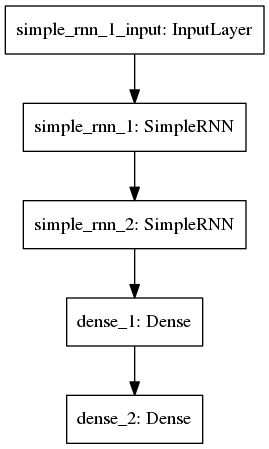
\includegraphics[scale=0.6]{model_simple}
		\caption{RNN implementation}
		\label{audacity}
	\end{center}
\end{figure}




\newpage

\section{SOFTWARE DEVELOPMENT METHODOLOGY}
\subsection{Software Development Life Cycle}
A software development methodology or system development methodology is a framework that is used to structure, plan, and control the process of developing a software system. It is the practice of using selected process techniques to improve the quality of a software development effort. The documented collection of policies, processes and procedures used by a development team or organization to practice software engineering is called its software development methodology (SDM) or system development life cycle (SDLC). For the timely and successful implementation of any project one must follow a suitable software development model. For the purpose of our project we followed an incremental software building model as our project consists of several functional components to be developed in a incremental manner. In incremental model, the whole requirement is divided into various builds. During each iteration, the development module goes through the requirements, design, implementation and testing phases. Each subsequent release of the module adds function to the previous release. The process continues till the complete system is ready as per the requirement. It starts with a simple implementation of a subset of the software requirements and iteratively enhances the evolving versions until the full system is implemented. At each iteration, design modifications are made and new functional capabilities are added. The basic idea behind this method is to develop a system through repeated cycles  and in smaller portions at a time.
\begin{figure}[h]
	\begin{center}
		
		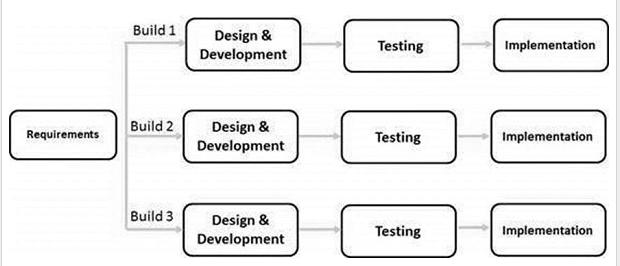
\includegraphics[scale=0.6]{SDLC.png}
		\caption{An Incremental Approach for Software Development}
		\label{SDLC}
	\end{center}
\end{figure}

Some of the basic characteristics of this software development methodology are:
\begin{itemize}
	\item Major requirements are defined; however, some functionalities or requested enhancements may evolve with time.
	\item Some working functionality can be developed quickly and early in the life cycle.
	\item Results are obtained early and periodically.
	\item Parallel development can be planned.
	\item Less costly to change the scope/requirements.
	\item Risk analysis is better and it supports changing requirements.
	\item Partial systems are built to produce the final system.
\end{itemize}

By following this model, we focused on building several components of the system in an incremental basis and finally those components are merged together to form a total functional system of Interactive voice response system with speech recognition module.


\subsection{Requirement Analysis}
Requirements analysis, also called requirements engineering, is the process of determining user expectations for a new system that is going to be build. These features, called requirements, must be quantifiable, relevant and detailed. In software engineering, such requirements are often called functional specifications. Requirements analysis is an important aspect of project management.
Requirements analysis involves frequent communication with system users to determine specific feature expectations, resolution of conflict or ambiguity in requirements as demanded by the various users or groups of users, avoidance of feature creep and documentation of all aspects of the project development process from start to finish. Energy should be directed towards ensuring that the final system or product conforms to client needs rather than attempting to mold user expectations to fit the requirements. Requirements analysis is a team effort that demands a combination of hardware, software and human factors engineering expertise as well as skills in dealing with people.

\subsubsection{Functional Requirements}

Functional requirements explain what has to be done by identifying the necessary task, action or activity that must be accomplished. In our project the core functional requirements can be as depicted in below:
\begin{enumerate}
	\item The system must be able to classify a voice signal from an independent speaker.
	\item The system must involve a significant degree of user interaction.
	\item The system must be able to run on different cross platforms.
	\item The system should allow the real time voice input by the user.
	\item The system must be capable of removing the potential noise effects on input voice signal
	
\end{enumerate}

\subsubsection{Non-Functional Requirements}
Non-functional requirements are requirements that specify criteria that can be used to judge the operation of a system, rather than specific behaviors. The non-functional requirements of the project  are listed below:

\begin{enumerate}
	\item The training of the sound samples must be effective and efficient.
	\item Mechanism of training sample generation must be easy and fast.
	\item The integration of all the system modules that compose a system must be easier and effective.
	\item The feedback from the system must be quick and in real time to make user feel in control during the interaction.
	
	
	
\end{enumerate}


\subsection{Feasibility Study}
Speech Recognition is one of the hottest topic in the current field of technology and science. Many researches have been carried out in this field from several decades ago to till today and many of them are still under study to optimize the study. The ASR system have been utilized in several sectors and have proved their importance in today\textquotesingle s technological world. By undertaking this project our attempt is to make use of speech recognition in a simple interactive system to automate the task using the voice command. We have undergone through several feasibility studies to make sure that the project is feasible and be developed . Some study topics are discussed below:


\subsubsection{Technical Feasibility}
ASR have been utilized under several platforms and several development approaches have been developed. Development of new artificial intelligence and pattern matching models have made it more simpler for implementation of ASR embedded with interactive system. Similarly today\textquotesingle s powerful computing processors and easy data collection software makes it more technically feasible.
\subsubsection{Operational Feasibility}
Many researches have been carried out in the field interactive systems using ASR most of which using English language. Such systems have proved to be easily operable several platforms. Our project is just a kind of implementation of ASR to automate task through Nepali voice . Thus this makes it operationally feasible for development.
\subsubsection{Economic Feasibility}
The project is economically feasible to begin with as no expensive hardware and software components is required. Similarly all the tools and techniques to be used are open source and are easily available free of cost. Data collection is done among us and other individuals which is economically feasible.
\subsubsection{Schedule  Feasibility}
To develop the project a proper time line has been projected to complete relevant portion of the project in scheduled time period. Most of the Necessary resources are  searched on the web and are available to begin research in time. Also all the related software packages are easily available which makes if more feasible.

\subsection{System Design}
\subsubsection{Use Case Diagram}

\begin{figure}[H]
	\begin{center}
		
		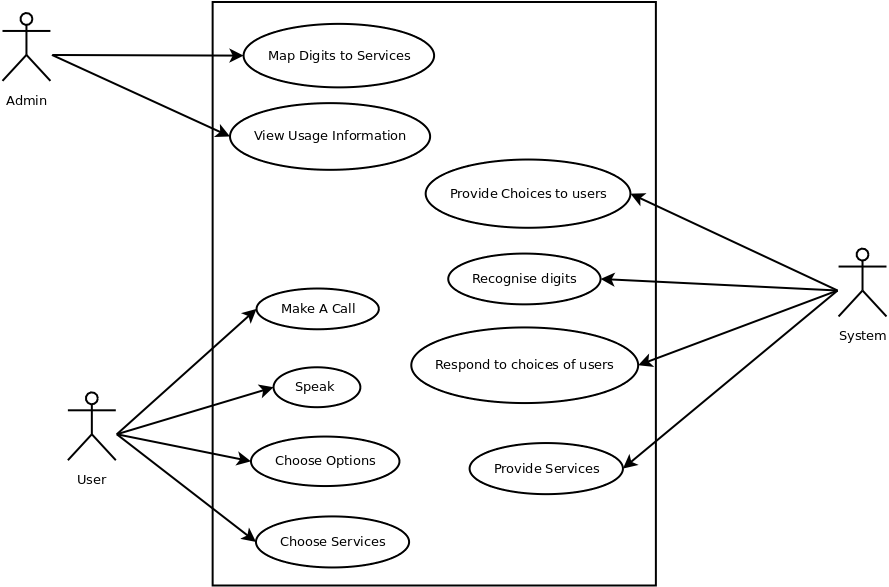
\includegraphics[width = \linewidth]{Usecase}
		\caption{Use Case Diagram}
	\end{center}
\end{figure}
\subsubsection{Sequence Diagram}
\begin{figure}[H]
	\begin{center}
		
		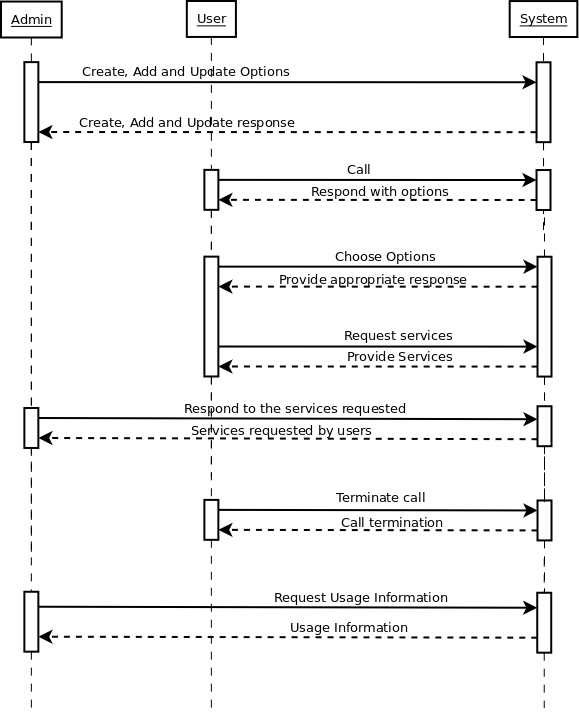
\includegraphics[scale = 0.5]{sequence}
		\caption{Sequence Diagram}
	\end{center}
\end{figure}

\subsubsection{Data Flow Diagram}
\begin{figure}[H]
	\begin{center}
		
		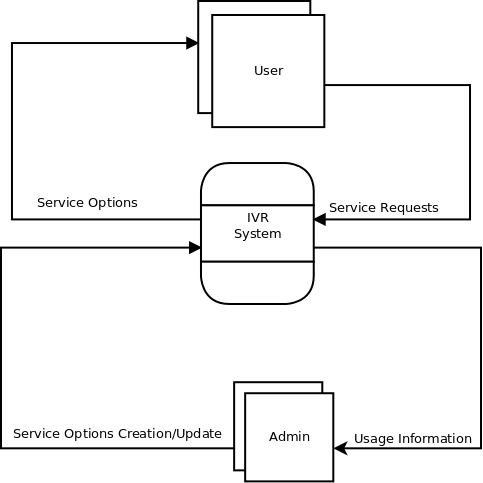
\includegraphics[scale = 0.5]{DFD}
		\caption{Data Flow Diagram}
	\end{center}
\end{figure}
\subsection{Tools and Technologies}
\subsubsection{Python Programming Language}
Python is a general-purpose, open source computer programming language. It is optimized for software quality, developer productivity, program portability, and component integration. Python is used by at least hundreds of thousands of developers around the world in areas such as internet scripting, systems programming, user interfaces, product customization, numeric programming, and more. It is generally considered to be among the top four or five most widely-used programming languages in the world today.

As a popular language focused on shrinking development time, python is deployed in
a wide variety of products and roles. Counted among its current user base are Google,
YouTube, industrial light and magic, esri, the bit torrent file sharing system, NASA\textquotesingle s
jet propulsion lab, the game eve online, and the national weather service. Python\textquotesingle s
application domains range from system administration, website development, cell
phone scripting, and education to hardware testing, investment analysis, computer games, and spacecraft control. Among other things, python sports a remarkably simple, readable, and maintainable syntax; integration with external components coded in other languages; a multiparadigm design, with OOP, functional, and modular structures; and a vast collection of precoded interfaces and utilities. Its tool set makes it a flexible and agile language,
ideal for both quick tactical tasks as well as longer-range strategic application development efforts. Python features a dynamic type system and automatic memory management and supports multiprogramming paradigms including object oriented, imperative, functional programming, and procedural styles. It has a large and comprehensive standard library. Python interpreters are available for many operating systems, allowing Python code to run on a wide variety of systems. Although it is a general-purpose language, python is often called a scripting language because it makes it easy to utilize and direct other software components. Perhaps python\textquotesingle s best asset, though, is simply that it makes software development more rapid and enjoyable. 

The major reasons behind the use of python programming language for this project are discussed below in brief.
\begin{itemize}
	\item Software quality:
	
	For many, Python\textquotesingle s focus on readability, coherence, and software quality in general
	sets it apart from other tools in the scripting world. Python code is designed to be
	readable, and hence reusable and maintainable much more so than traditional
	scripting languages. The uniformity of Python code makes it easy to understand,
	even if you did not write it. In addition, Python has deep support for more advanced
	software reuse mechanisms, such as object-oriented programming (OOP) and function programming.
	
	\item Developer productivity:
	
	Python boosts developer productivity many times beyond compiled or statically
	typed languages such as C, C++, and Java. Python code is typically one-third to
	one-fifth the size of equivalent C++ or Java code. That means there is less to type, 
	less to debug, and less to maintain after the fact. Python programs also run immediately, without the lengthy compile and link steps required by some other tools, 
	further boosting programmer speed.
	
	\item Program Portability:
	
	Most Python programs run unchanged on all major computer platforms. Porting
	Python code between Linux and Windows, for example, is usually just a matter of
	copying a script\textquotesingle s code between machines. Moreover, Python offers multiple options for coding portable graphical user interfaces, database access programs, web based systems, and more. Even operating system interfaces, including program launches and directory processing are as portable is Python as they can possibly be.
	
	\item Support Libraries:
	
	Python comes with a large collection of pre-built and portable functionality, known
	as the standard library. This library supports an array of application-level programming tasks, from text pattern matching to network scripting. In addition,
	Python can be extended with both homegrown libraries and a vast collection of
	third-party application support software. Python \textquotesingle s third-party domain offers tools
	for website construction, numeric programming, serial port access, game development, and much . The NumPy extension, for instance, has been described as a free and more powerful equivalent to the Matlab numeric programming system.
	
	\item Component Integration:
	
	Python scripts can easily communicate with other parts of an application, using a
	variety of integration mechanisms. Such integrations allow Python to be used as a
	product customization and extension tool. Today, Python code can invoke C and
	C++ libraries, can be called from C and C++ programs, can integrate with Java
	and .NET components, can communicate over frameworks such as COM and Silverlight, can interface with devices over serial ports, and can interact over networks
	with interfaces like SOAP, XML-RPC, and CORBA. It is not a standalone tool.
\end{itemize}
\subsubsection{NumPy}
NumPy is the high performance numeric programming extension for python. It is the core library for scientific computing in Python. It is a Python library that provides a multidimensional array object, various derived objects (such as masked arrays and matrices), and an assortment of routines for fast operations on arrays, including mathematical, logical, shape manipulation, sorting, selecting, I/O, discrete Fourier transforms, basic linear algebra, basic statistical operations, random simulation and much more.

It contains among other things:

\begin{itemize}
	\item a powerful N-dimensional array object
	\item sophisticated (broadcasting) functions
	\item tools for integrating C/C++ and Fortran code
	\item useful linear algebra, Fourier transform, and random number capabilities
\end{itemize}

Besides its obvious scientific uses, NumPy can also be used as an efficient multi-dimensional container of generic data. Arbitrary data-types can be defined. This allows NumPy to seamlessly and speedily integrate with a wide variety of databases.
\subsubsection{PyAudio}
PyAudio provides Python bindings for PortAudio, the cross-platform audio I/O library. With PyAudio, you can easily use Python to play and record audio on a variety of platforms. PyAudio is inspired by:

\begin{itemize}
	\item pyPortAudio/fastaudio: Python bindings for PortAudio v18 API.
	\item tkSnack: cross-platform sound toolkit for Tcl/Tk and Python.
\end{itemize}

PyAudio provides Python bindings for PortAudio, the cross-platform audio I/O library. With PyAudio, you can easily use Python to play and record audio on a variety of platforms. PyAudio is inspired by:
pyPortAudio/fastaudio: Python bindings for PortAudio v18 API.
tkSnack: cross-platform sound toolkit for Tcl/Tk and Python.
To use PyAudio, we first instantiate PyAudio using pyaudio.PyAudio() , which sets up the portaudio system. To record or play audio, we open a stream on the desired device with the desired audio parameters using pyaudio.PyAudio.open() . This sets up a pyaudio.Stream to play or record audio.  We play audio by writing audio data to the stream using pyaudio.Stream.write(), or read audio data from the stream using pyaudio.Stream.read().
In "blocking mode" each pyaudio.Stream.write() or pyaudio.Stream.read() blocks until all the given/requested frames have been played/recorded. Alternatively, to generate audio data on the fly or immediately process recorded audio data, use the "callback mode". 

\subsubsection{Pomegranate}
pomegranate is a python package which implements fast, efficient, and extremely flexible
probabilistic models ranging from probability distributions to Bayesian networks to
mixtures of hidden Markov models. Pomegranate has been used in our project to create the
HMM models.	
\subsubsection{PyQT}
PyQt4 is a toolkit for creating GUI applications. It is a blending of Python programming language and the successful Qt library. Qt library is one of the most powerful GUI libraries. PyQt4 is developed by Riverbank Computing. 

PyQt4 is implemented as a set of Python modules. It has 440 classes and 6000 functions and methods. It is a multiplatform toolkit which runs on all major operating systems, including UNIX, Windows, and Mac OS. PyQt4 is dual licensed. Developers can choose between a GPL and a commercial license. Previously, GPL version was available only on UNIX. Starting from PyQt version 4, GPL license is available on all supported platforms.


PyQt4's classes are divided into several modules. Some of them are:
\begin{itemize}
	\item QtCore
	\item QtGui
	\item QtNetwork
	\item QtXml
	\item QtSvg
	\item QtOpenGL
	\item QtSql
\end{itemize}
The QtCore module contains the core non GUI functionality. This module is used for working with time, files and directories, various data types, streams, URLs, mime types, threads or processes. The QtGui module contains the graphical components and related classes. These include for example buttons, windows, status bars, toolbars, sliders, bitmaps, colours, and fonts. The QtNetwork module contains the classes for network programming. These classes facilitate the coding of TCP/IP and UDP clients and servers by making the network programming easier and more portable. The QtXmlcontains classes for working with XML files. This module provides implementation for both SAX and DOM APIs. The QtSvg module provides classes for displaying the contents of SVG files. Scalable Vector Graphics (SVG) is a language for describing two-dimensional graphics and graphical applications in XML. The QtOpenGL module is used for rendering 3D and 2D graphics using the OpenGL library. The module enables seamless integration of the Qt GUI library and the OpenGL library. The QtSql module provides classes for working with databases.

\subsubsection{TensorFlow}

TensorFlow is an open source software library for numerical computation using data flow graphs. Nodes in the graph represent mathematical operations, while the graph edges represent the multidimensional data arrays (tensors) communicated between them. The flexible architecture allows us to deploy computation to one or more CPUs or GPUs in a desktop, server, or mobile device with a single API. TensorFlow was originally developed by researchers and engineers working on the Google Brain Team within Google's Machine Intelligence research organization for the purposes of conducting machine learning and deep neural networks research, but the system is general enough to be applicable in a wide variety of other domains as well. 

\subsubsection{keras}

Keras is a high-level neural networks API, written in Python and capable of running on top of TensorFlow, CNTK, or Theano. It enables  fast experimentation.

\subsection{Project Scheduling}

\begin{figure}[H]
	\begin{center}
		
		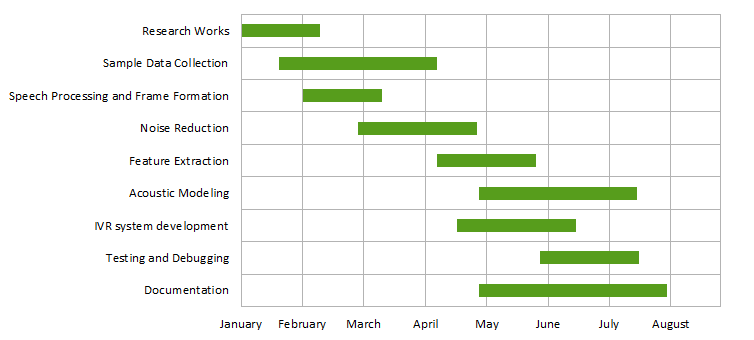
\includegraphics[width = \linewidth]{gantt}
		\caption{Gantt Chart for Project}
	\end{center}
\end{figure}

\newpage

\section{RESULTS AND VALIDATION}
The final result of the system being developed is a desktop environment where user can interact with the system through voice command to accomplish the task. The current system consists of simple GUI in the desktop environment that greets user with the greeting message at the welcome screen and then prompts the user to choose one of the available service options using his voice command which in our case is done by using the Nepali Numeral words. Based on the voice command i.e. the number spoken by user typical service is chosen and the response system selects the service option with the number being assigned to it.

The result thus obtained is being analyzed in context of several parameters of the system during various development phases.Result of several phases have been studied and analyzed as discussed below using appropriate constraints of the measurement that are depicted below
in detail.

\subsection{Result}

\subsubsection{Data Sample}
For our project we used Nepali numeral words recognition in order to embed with the interactive response system. Thus for the training of the system training data sets were required. Due to unavailability of data samples we collected the samples from different individuals through a recording software. The details regarding the data samples are tabulated in a table given below:


\begin{center}
	\begin {table}[h]
	\begin{center}
		
	\begin{tabular}{ |c|c| } 
		\hline
		Total number of Samples & 100 Samples per word  \\ 
		\hline
		Recorded Sample Frequency & 16000 Hz  \\ 
		\hline
		Number of Speakers & 20  \\ 
		\hline
	\end{tabular}
\caption{Test data sample details}
\end{center}
\end{table}
\end{center}


\subsubsection{Noise Reduction}

We used Spectral Subtraction method to reduce the additive noise from the speech signal. Based on testing the various level of threshold, we we able to remove the additive noise from the signal and have a mostly clean signal.


Below image shows a noisy signal and the clean noise reduced signal.

\begin{figure}[H]
	\begin{center}
		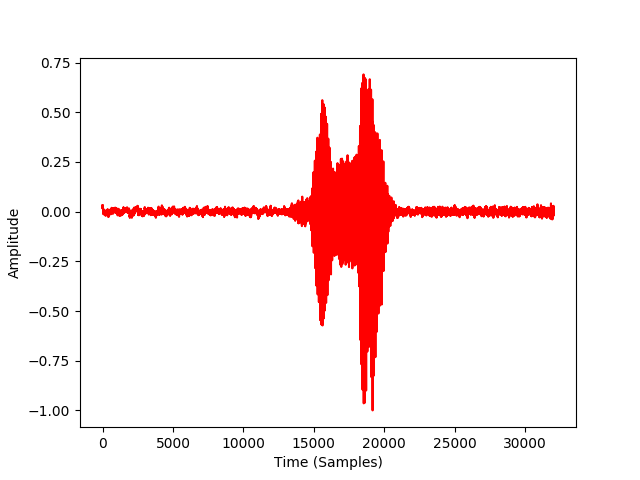
\includegraphics[scale=0.8]{images/mainSigOriginal.png}
		\caption{Original Sound Signal}
		\label{original sound}
	\end{center}
\end{figure}

\begin{figure}[H]
	\begin{center}
		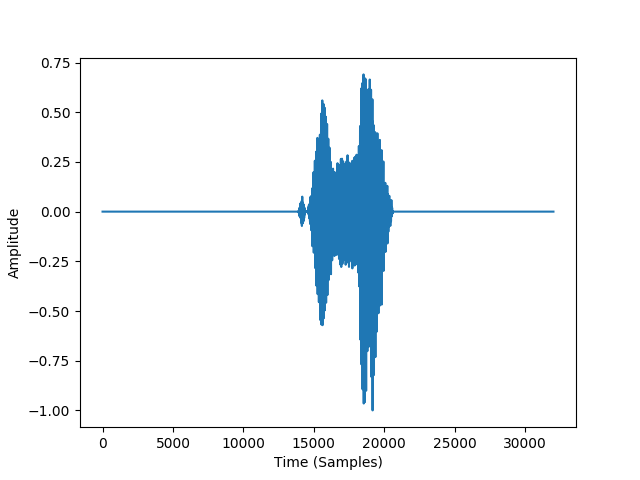
\includegraphics[scale=0.8]{images/mainSigRefine.png}
		\caption{Refined Sound Signal}
		\label{refined sound}
	\end{center}
\end{figure}



The spectrogram below shows the spectral subtraction of average noise.
\begin{figure}[H]
	\begin{center}
		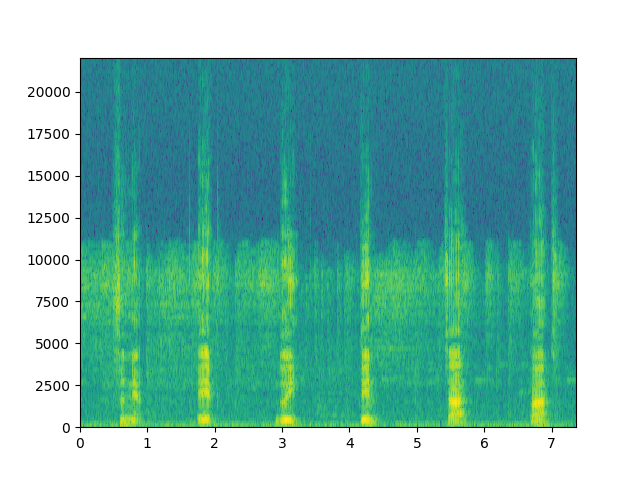
\includegraphics[scale=0.5]{images/main_Spectogram_Original.png}
		\caption{Spectogram of Original Sound Signal}
		\label{Spectro_original}
	\end{center}
\end{figure}

\begin{figure}[h]
	\begin{center}
		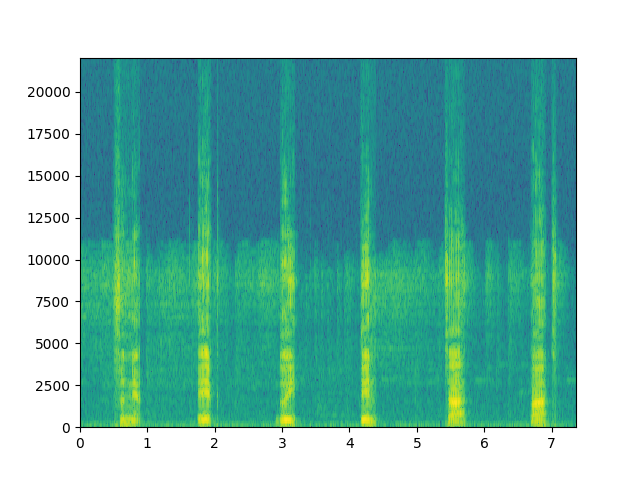
\includegraphics[scale=0.7]{images/MainSpectogram_Refine.png}
		\caption{Spectogram of Refined Sound Signal}
		\label{Spectro_refined}
	\end{center}
\end{figure}


\subsubsection{Silence Removal Module}
	
	During the training sample generation and actual testing, we trimmed away the silence part and extracted only the voiced region. By breaking the sample into chunks and based on the threshold level, we extracted only the voiced sound. 
	
	Below shows the original image and another only the voiced image with trimmed initial and ending silences.
	
	\begin{figure}[H]
		\begin{center}
			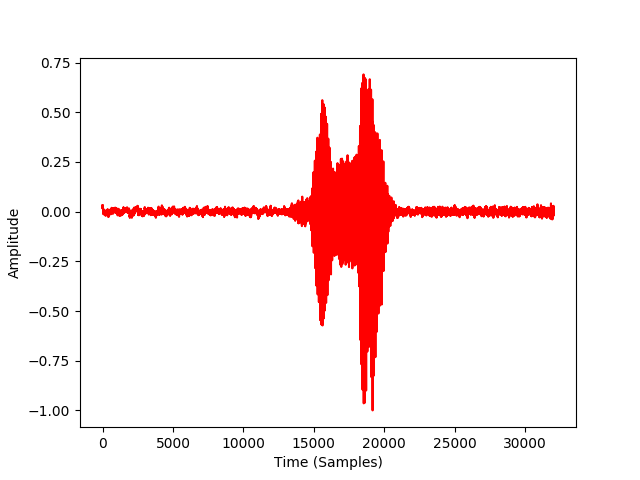
\includegraphics[scale=0.8]{images/mainSigOriginal.png}
			\caption{Original input sound signal}
			\label{orginal}
		\end{center}
	\end{figure}
	
	
	\begin{figure}[H]
		\begin{center}
			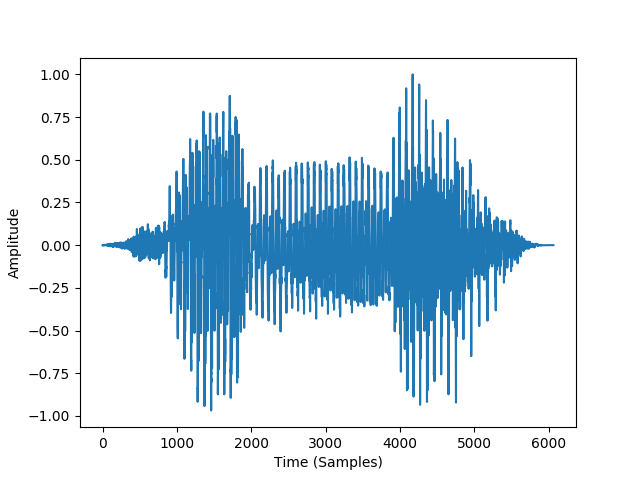
\includegraphics[scale=0.8]{images/voiced_sound.png}
			\caption{Voiced sound signal}
			\label{Voiced}
		\end{center}
	\end{figure}
	
	
	

\subsubsection{HMM Module}


The Output for any speech signal in an HMM module is the probability that the speech signal belongs to that model. We have created different HMM model for each word and the speech signal is passed through every model to predict what are its probability of being in that model. The probability calculated in the Log Probability.

\begin{figure}[H]
	\begin{center}
		
		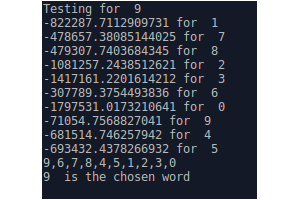
\includegraphics[scale = 1.0]{results_hmm}
		\caption{Log probability result for each model for a speech sample Nepali word 9}
	\end{center}
\end{figure}




\subsubsection{RNN Module}


Recurrent Neural Network can be applied in place of Hidden Markov Model. The output is the number that it predicts after it runs through the sequence of data.

\begin{figure}[H]
	\begin{center}
		
		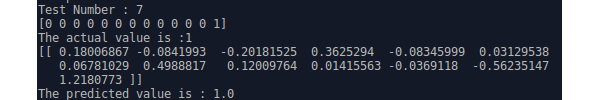
\includegraphics[scale = 0.5]{results_rnn}
		\caption{The result for a word speech of 1 in a RNN module}
	\end{center}
\end{figure}



\subsubsection{Output of the System}

The Result of the overall project is an Interactive Voice Response System. The IVR system is implemented as a desktop application where the user is given a list of options and he can navigate through the options using his speech as input. The system is an overall integration
of Noise Reduction Module, Silence Removal Module, Feature Extraction Module and a prediction module for which either HMM Module or RNN Module can be used.

\begin{figure}[H]
	\begin{center}
		
		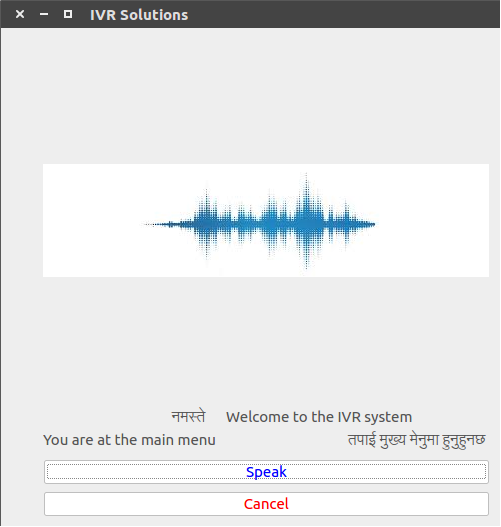
\includegraphics[scale = 0.4]{mainpage}
		\caption{The first GUI interface of the system}
	\end{center}
\end{figure}

\begin{figure}[H]
	\begin{center}
		
		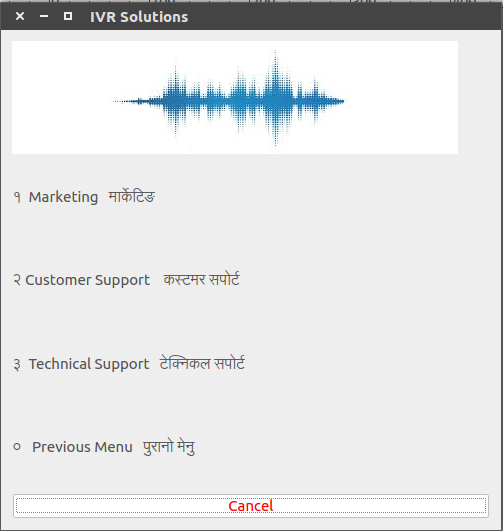
\includegraphics[scale = 0.4]{secondpage}
		\caption{The interface where voice input can be provided to make a selection}
	\end{center}
\end{figure}

\begin{figure}[H]
	\begin{center}
		
		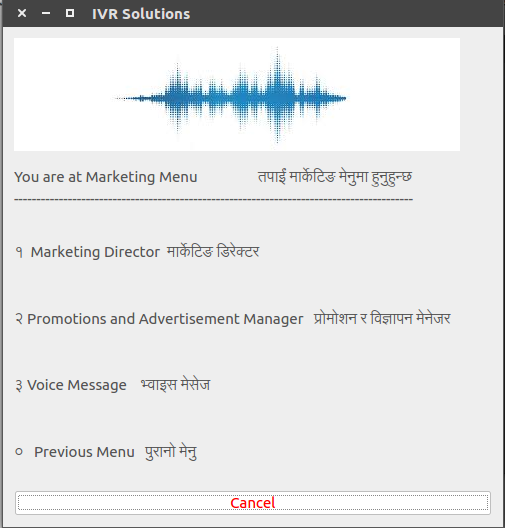
\includegraphics[scale = 0.4]{thirdpage}
		\caption{The interface after the selection has been made where there are again list of options}
	\end{center}
\end{figure}


\subsection{Validation}

The system was validated by checking the number of times it makes the correct prediction for the samples given. The system is an overall integration of Noise Reduction Module, Silence Removal Module, Feature Extraction Module and a prediction module for which either HMM Module or RNN Module can be used. For the initial phase HMM module was chosen as the prediction module.

The approach taken for validation was dividing the samples that we had into training samples and test samples to check how many correct predictions does the sample makes. We used one sample from each word as test data and were able to get an accuracy of around 70 percentage.

\begin{figure}[H]
	\begin{center}
		
		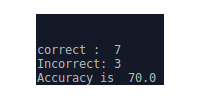
\includegraphics[scale = 1.0]{hmm_accuracy}
		\caption{Accuracy for Test Samples using HMM Module for Prediction}
	\end{center}
\end{figure}

Now the next approach applied for validating the HMM result was by using the live user data to be feed into the HMM. The accuracy was calculated by calculating the total times the HMM model makes correct predictions out of total number of data feed in. In this approach the total accuracy was around 76 percentage.
We can now validate the use of noise reduction module and Silence Removal module using the same system as above . For both Noise Reduction Module and Silence Removal Module, a same approach was take, the system was ran once with the modules in them and once without them and the accuracy were compared.

\begin{center}
	\begin {table}[h]
	\begin{center}
		
		\begin{tabular}{ |c|c| } 
			\hline
			\textbf{Without Noise Reduction Module} & \textbf{With Noise Reduction Module}  \\ 
			\hline
			60.12\% & 74.28\%  \\ 
			\hline
		
		\end{tabular}
		\caption{Accuracy Comparison for Use of Noise Reduction Module}
	\end{center}
\end{table}
\end{center}


\begin{center}
	\begin {table}[h]
	\begin{center}
		
		\begin{tabular}{ |c|c| } 
			\hline
			\textbf{Without Silence Removal Module} & \textbf{With Silence Removal Module}  \\ 
			\hline
			52.12\% & 74.28\%  \\ 
			\hline
			
		\end{tabular}
		\caption{Accuracy Comparison for use of Silence Removal Module}
	\end{center}
\end{table}
\end{center}

Now, we can run similar kind of test while using the RNN prediction module. RNN can be used instead of HMM to use it as a prediction module. We need to first select among the various RNN implementations available. We have got Simple RNN, LSTM RNN and GRU RNN. A test for all these three was run.

\begin{figure}[H]
	\begin{center}
		
		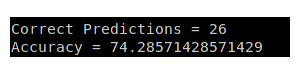
\includegraphics[scale = 0.5]{simple_result}
		\caption{The accuracy while using Simple RNN}
	\end{center}
\end{figure}
\begin{figure}[H]
	\begin{center}
		
		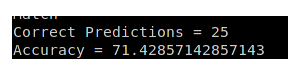
\includegraphics[scale = 0.5]{lstm_result}
		\caption{The accuracy while using LSTM RNN}
	\end{center}
\end{figure}

\begin{figure}[H]
	\begin{center}
		
		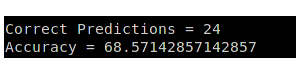
\includegraphics[scale = 0.5]{gru_result}
		\caption{The accuracy while using GRU RNN}
	\end{center}
\end{figure}

\begin{center}
	\begin {table}[h]
	\begin{center}
		
		\begin{tabular}{ |c|c| } 
			\hline
			\textbf{RNN Module} & \textbf{Accuracy}  \\ 
			\hline
			Simple RNN & 74.28\%  \\ 
			\hline
			LSTM & 71.43\%  \\ 
			\hline
			GRU & 68.57\%  \\ 
			\hline			
		\end{tabular}
		\caption{Accuracy Comparison for Various Variations of RNN}
	\end{center}
\end{table}
\end{center}

Now test were run to identify the perfect number of hidden units in the layers. The test was carried out by using various numbers of hidden units to find the optimal one.

\begin{figure}[H]
	\begin{center}
		
		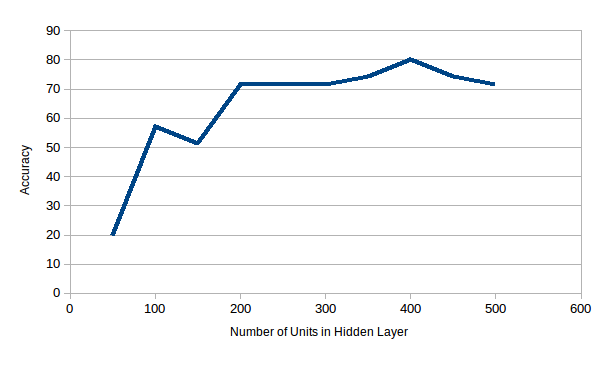
\includegraphics[width = \linewidth]{comparison_rnn}
		\caption{Accuracy for Various number of Hidden Units}
	\end{center}
\end{figure}




\subsection{Analysis}

From Above results, we can see that the use of Noise Reduction Module and Silence Detection Module gave good accuracy when they were used as compared to when they were not used and are so an integral part of the system. The accuracy of HMM module is good given the fact that we had such a small dataset available and same is the case with RNN module being used.

We got that Simple RNN has better accuracy then GRU and LSTM. Though LSTM and GRU are advancements of Simple RNN, the accuracy of RNN was still high due to the fact that our model is a simple kind of RNN models with not much dependencies so Simple RNN performed better. The Number of hidden units with 400 gave the best result and thus the same one was used for further processing. The best accuracy of 80 percentage while
using simple RNN and 400 hidden cell units was obtained. The accuracy of RNN is better compared to HMM.

The best accuracy that we could obtain was only of 80 percentage. Though this accuracy is less compared to above 95 perecentage accuracy obtained by Google, Baidu, Etc, but our accuracy can be considered fairly good based on the fact that we had a limited number os samples. The accuracy of our system will increase if we can generate more samples.

\newpage

\section{CONCLUSION}
Speech Recognition has become very important in today's world. With the advancements in technology and improvements in recognition algorithms, speech has become one of the primary source of input for many applications. Speech is the most efficient and natural way of communication. So, it is intuitive that speech recognition systems have found applications in various fields. 

Interactive Voice Response (IVR) systems are one of the prominent systems that have a huge potential for use of voice signals as input to the system. With this in mind, we presented an idea for the development of an IVR system with Automatic Speech Recognition (ASR). The initial objective of the project was to develop a system capable of recognizing voice signals in Nepali Language input to the IVR system. Throughout the course of the development phase, various limitations and obstacles were encountered which prompted us to develop the system capable of recognizing words corresponding to the digits of the Nepali Language. For this, we researched on various methods of speech recognition and used the findings of these researches to develop the system. 

The project was implemented by using algorithms like Noise Reduction, Voice Activity Detection, MFCC Feature Extraction, Hidden Markov Model and Recurrent Neural Network. The overall accuracy of the system while using HMM was around 70 percentage and while using RNN was around 80 percentage. The greater accuracy of RNN is due to the fact that, RNN do not make Markov assumptions and can account for long term dependencies when modeling natural language and due to the the greater representational power of neural networks and their ability to perform intelligent smoothing by taking into account syntactic and semantic features. Though the accuracy seems to be a bit less, the accuracy is good compared to the fact that we had such less data set available. With proper amount of data set available the project can get much higher accuracy and can be implemented.




\newpage

\section{LIMITATIONS AND FURTHER WORKS}
Speech Recognition has been a very interesting field in research and technology.Many technical teams around the globe are working together to get the satisfactory result.Several researches are ongoing in this field and due to advancement in technology and efficient new models it has made possible to make further enhancement in this field to get more accurate results.Like many other projects our project has also got limitations and the enhancements that can be made in future.

\subsection{Limitations}
Some of the particular field of limitations  are:
\begin{enumerate}
	\item \textbf{Narrow Recognition Domain: }
	Currently the IVR system with speech recognition system works on very narrow domain. Because of time limitation and difficulty in collecting the data samples at present we are focused on using only Nepali numbers from zero to nine in the system.The accuracy level of recognition is dependent on available number of training samples but due to unavailability of training data only fewer data are being trained and recognized.
	\item \textbf{Offline operation: }
	Another limitation of the current system is that it is 
	designed only for the offline operation i.e. available only on desktop environment but not on the web.
	\item \textbf{Narrow application domain: }
	Our present system is focused only in implementation speech recognition on automating a simple task in desktop environment.
	
	
\end{enumerate}

\subsection{Future Enhancements}
The potential enhancements that can be made to the system are discussed below:
\begin{enumerate}
	\item By increasing the training data samples using effective data collection mechanism the domain of recognition can be increased.
	\item The system may be enhanced to make work for online mode by integrating it in web applications.
	\item The system can be enhanced to apply on the real time applications using telephone. For this further research on particular domain is necessary.
\end{enumerate}






\newpage
\phantomsection \addcontentsline{toc}{section}{REFERENCES}
\renewcommand{\refname}{REFERENCES}
\bibliographystyle{unsrt}
\bibliography{main}

%\printbibliography


\nocite{c-olah:lstm, a-kar:rnn-effectiveness, malay-rnn, wiki:hmm, wiki:markov, machine-learning-mastery, avash-nepalispeech, tanlee-isolate, isolated-simple-rnn, arabic-rnn, SpectralSub:Tutorial, Noise_Reduction, spectral-article, noise_reduce, Spec:Tutorial, Pydubs, Spectral:Demo,Numpy:Docs, j-lyons:features,feature-extraction,techniques-feature}

\end{document}
